% ============================================================
%  Audio Amplifier Design Report – EW-II Project 1, Table 28
%  Two-column IEEE-style format
% ============================================================
\documentclass[10pt,twocolumn]{article}

% ── Packages ──
\usepackage[a4paper,margin=1.8cm,top=2cm,bottom=2cm]{geometry}
\usepackage{graphicx}
\usepackage{amsmath,amssymb}
\usepackage{booktabs}
\usepackage{caption}
\usepackage{subcaption}
\usepackage{hyperref}
\usepackage{enumitem}
\usepackage{fancyhdr}
\usepackage{float}
\usepackage{siunitx}
\usepackage{circuitikz}
\usepackage{tabularx}
\usepackage{titlesec}
\usepackage{xcolor}

% ── Custom Colors ──
\definecolor{headblue}{HTML}{1F4E79}
\definecolor{iitblue}{RGB}{0,84,166}
\definecolor{lightgray}{RGB}{245,245,245}
\definecolor{darkgray}{RGB}{80,80,80}

% ── Page Style ──
\pagestyle{fancy}
\fancyhf{}
\fancyhead[L]{ 2024102014 \& 2024102054}
\fancyhead[R]{ EW-II Project 1 \textbar\ Audio Amplifier}
\fancyfoot[C]{\thepage}
\renewcommand{\headrulewidth}{0.4pt}

% ── Section Formatting ──
\titleformat{\section}{\large\bfseries\color{iitblue}}{}{0em}{\thesection\quad}[\titlerule]
\titleformat{\subsection}{\normalsize\bfseries\color{darkgray}}{}{0em}{\thesubsection\quad}
\titleformat{\subsubsection}{\normalsize\itshape}{}{0em}{\thesubsubsection\quad}

% ── Hyperref ──
\hypersetup{colorlinks=true,linkcolor=blue!60!black,citecolor=green!50!black,urlcolor=blue!70!black}

\graphicspath{{images/}}

% ============================================================
\begin{document}

% ──────────────────────────────────────────────────────────────
%  TITLE (spans both columns)
% ──────────────────────────────────────────────────────────────
\twocolumn[{%
\begin{center}
    % Uncomment the next line if you have an institute logo:
    % \includegraphics[width=3cm]{images/institute_logo.png}\\[6pt]
    {\LARGE\bfseries\color{iitblue} Audio Amplifier Design and Implementation}\par\vspace{4pt}
    {\large EW-II Project 1 \textbar\ Table No.\ 5 \textbar\ Room N-104}\par\vspace{10pt}
    \begin{tabular}{c c c}
        \textbf{Name} & \textbf{Roll No.}  \\
        \midrule
        Akshay Chanda       & 2024102014 \\
        S V Santhosh Yadav  & 2024102054 \\
    \end{tabular}\par\vspace{6pt}
    {\normalsize International Institute of Information Technology, Hyderabad (IIIT-H)}
\end{center}
\vspace{8pt}
\hrule
\vspace{10pt}
}]

% ──────────────────────────────────────────────────────────────
%  ABSTRACT / AIM
% ──────────────────────────────────────────────────────────────
\section{Aim}
To design and build an audio amplifier satisfying the specifications in Table~\ref{tab:specs}.

\begin{table}[H]
\centering
\caption{Design Specifications}
\label{tab:specs}
\small
\begin{tabularx}{\linewidth}{lX}
\toprule
\textbf{Parameter}          & \textbf{Value} \\
\midrule
Supply voltage              & $\pm 5\;\text{V}$ \\
Supply voltage              & $\pm 12\;\text{V}$ (Op-amp) \\
Input signal                & $10$--$20\;\text{mV}_{pp}$ \\
Voltage gain (Pre-amp + CE) & $ \sim 450 $ \\
Frequency range             & $20\;\text{Hz}$--$20\;\text{kHz}$ \\
Output power                & $= 0.98 \;\text{W}$ \\
Filter attenuation          & $0\;\text{dB}$ in passband \\
Power amp voltage gain      & Unity ($\times 1$) \\
Load impedance              & $\geq 10\;\Omega$ \\
\bottomrule
\end{tabularx}
\end{table}

The amplifier chain consists of four cascaded stages:
\begin{enumerate}[nosep]
    \item Differential pre-amplifier (gain $G_1 \geq 2$)
    \item Common-emitter gain stage (gain $G_2$, with $G_1 \cdot G_2 \geq 500$)
    \item Band-pass filter (20\,Hz -- 20\,kHz, unity gain)
    \item Class-AB power amplifier (unity voltage gain)
\end{enumerate}

% ══════════════════════════════════════════════════════════════
\section{Power Supply and Input Stage}
% ══════════════════════════════════════════════════════════════

\subsection{Voltage Regulators: LM7805 and LM7905}
Stages 1, 2, and 4 operate from a regulated dual supply of $\pm5\;\text{V}$.
This is derived using two fixed-voltage linear regulators:

\begin{itemize}[nosep]
    \item \textbf{LM7805} — positive regulator, outputs $+5\;\text{V}$.
    \item \textbf{LM7905} — negative regulator, outputs $-5\;\text{V}$.
\end{itemize}

Stage 3 (UA741 op-amp) requires a wider supply for adequate headroom and slew rate.
It is powered directly from $\pm12\;\text{V}$ rails without regulation down to $\pm5\;\text{V}$.

\noindent\textbf{Why regulated supply?}
Unregulated DC from a transformer-rectifier has ripple that adds hum to the amplified signal.
The LM7805/LM7905 provide clean, stable $\pm5\;\text{V}$ regardless of load current variations,
ensuring consistent biasing across all transistor stages.

\noindent\textbf{LM7805 (positive regulator):}
Input voltage range: $7\;\text{V}$ to $35\;\text{V}$. Output: $+5\;\text{V}$ at up to $1\;\text{A}$.
Requires $0.1\;\mu\text{F}$ bypass capacitor at the output for stability.

\noindent\textbf{LM7905 (negative regulator):}
Input voltage range: $-7\;\text{V}$ to $-35\;\text{V}$. Output: $-5\;\text{V}$ at up to $1\;\text{A}$.
Pin order differs from the 7805 (input and common are swapped), so care is taken during wiring.

\begin{figure}[H]
    \centering
    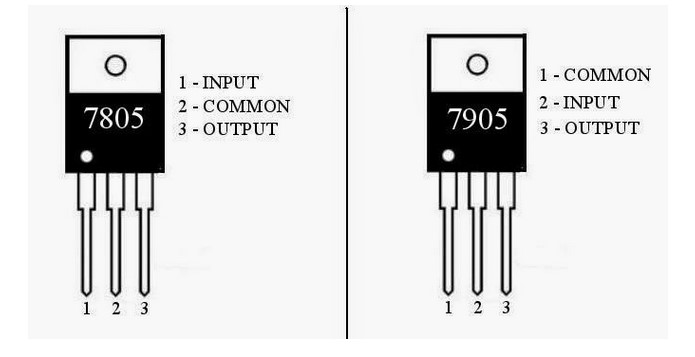
\includegraphics[width=0.85\linewidth]{images/regulator_pinout.png}
    \caption{LM7805 and LM7905 combined pinout diagram showing pin assignments.}
    \label{fig:reg_pinout}
\end{figure}

\begin{figure}[H]
    \centering
    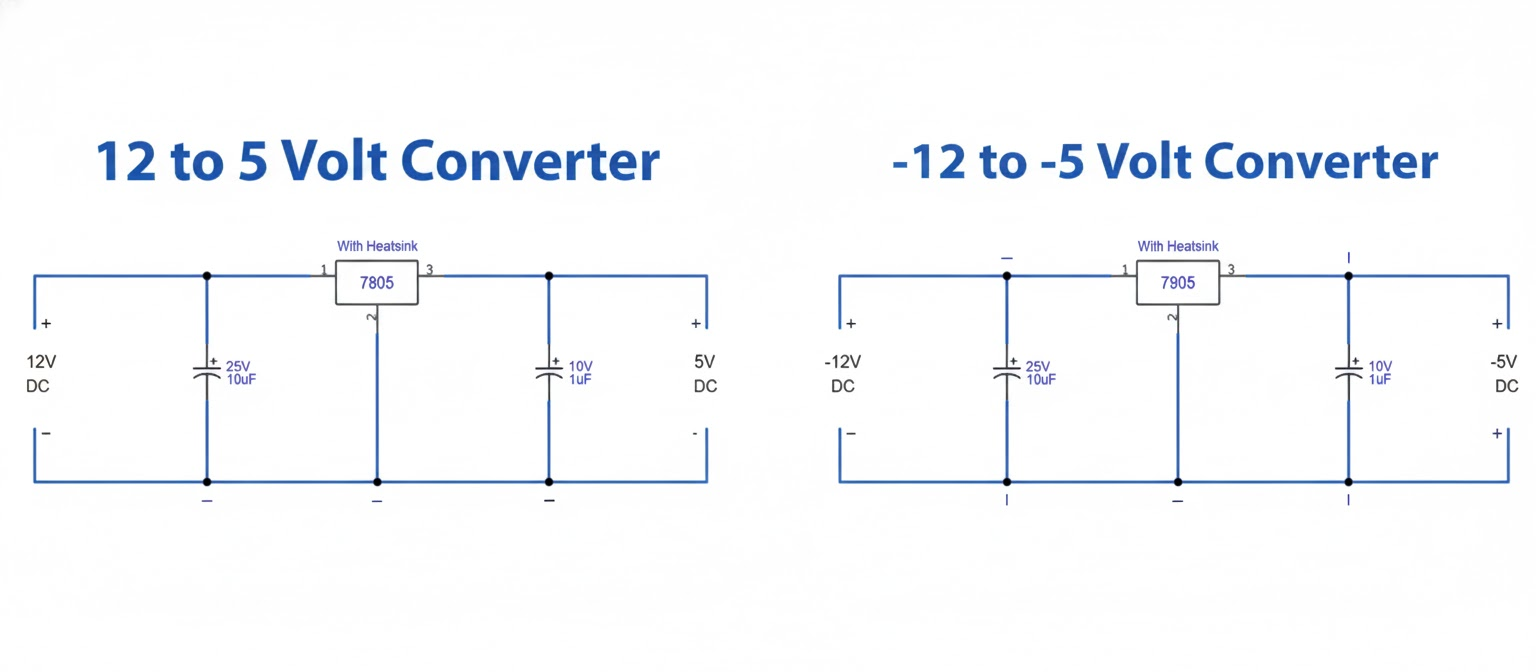
\includegraphics[width=0.85\linewidth]{images/regulator_circuit.png}
    \caption{Combined power supply circuit: LM7805 and LM7905 regulators providing
             $\pm5\;\text{V}$ to Stages 1, 2, and 4.}
    \label{fig:reg_circuit}
\end{figure}

\subsection{Microphone Input Circuit}
A \textbf{condenser (electret) microphone} is used as the input source. It requires a small
DC bias current through a series resistor to power its internal FET.
The AC audio signal is then coupled via a capacitor to the amplifier input,
blocking the DC bias from entering Stage 1.

\begin{figure}[H]
    \centering
    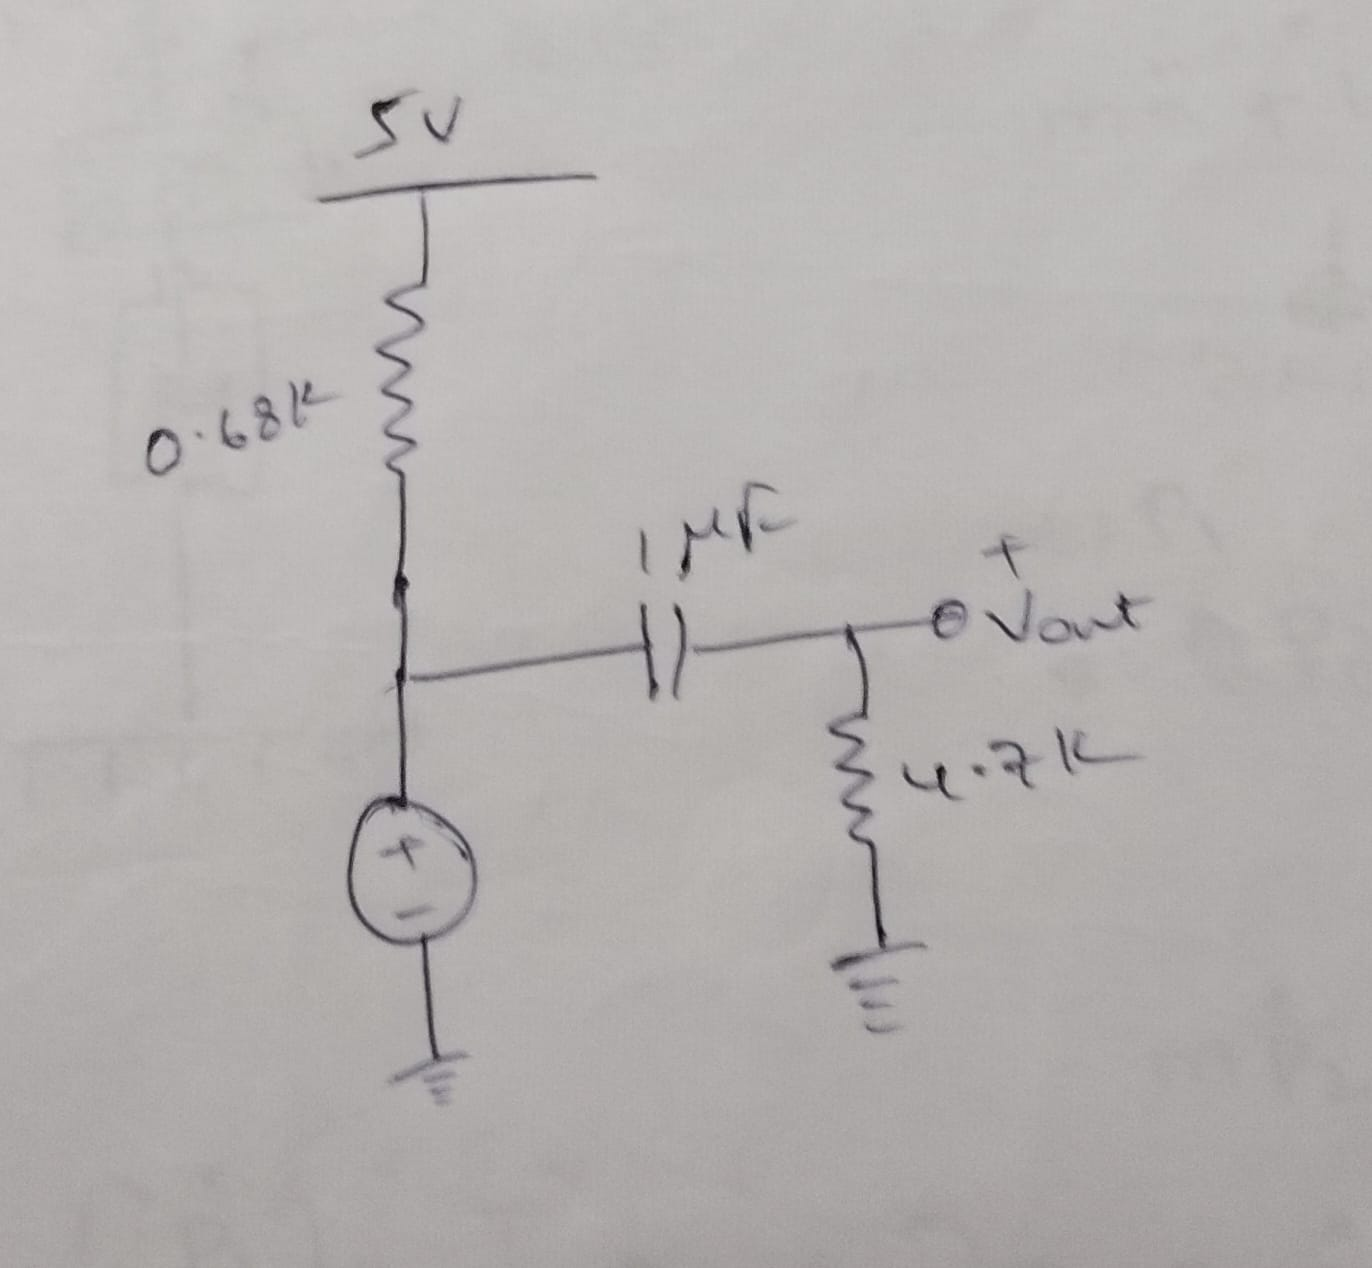
\includegraphics[width=0.85\linewidth]{images/mic_circuit.png}
    \caption{Microphone bias and coupling circuit feeding the input of Stage 1.}
    \label{fig:mic_circuit}
\end{figure}

% ══════════════════════════════════════════════════════════════
\section{Stage 1: Differential Pre-Amplifier}
% ══════════════════════════════════════════════════════════════

\subsection{Circuit Description}
The pre-amplifier uses a \textbf{common-emitter differential pair} built with two NPN BC547B transistors ($Q_1$, $Q_2$). A differential amplifier is chosen because it offers:
\begin{itemize}[nosep]
    \item \textbf{High input impedance} — prevents loading of the weak microphone signal.
    \item \textbf{Low output impedance} — enables efficient signal transfer to the next stage.
    \item \textbf{Good noise rejection} — common-mode noise is suppressed, preserving the integrity of the $10$--$20\;\text{mV}$ input.
\end{itemize}

For proper operation both BJTs must be in the \emph{active} region: base-emitter junction forward-biased and base-collector junction reverse-biased.

\subsection{Gain Derivation}
For a differential pair with an emitter degeneration resistor $R_E$ and collector resistors $R_{C1} = R_{C2} = R_C$, the differential-mode small-signal voltage gain is:
\begin{equation}
    A_d = \frac{v_{o}}{v_{id}} = \frac{-g_m R_C}{1 + g_m R_E / 2}
    \label{eq:diff_gain}
\end{equation}
where $g_m = I_C / V_T$ is the transconductance of each transistor.

\paragraph{Design values from the circuit:}
\begin{itemize}[nosep]
    \item $R_{C1} = R_{C2} = 390\;\Omega$
    \item $R_E = 1.075\;\text{k}\Omega$
    \item $V_{CC} = 5\;\text{V}$, $V_{EE} = -5\;\text{V}$
    \item Input: $V_{in} = 10\;\text{mV}$ peak, $f = 1\;\text{kHz}$ (single-ended)
\end{itemize}

The tail current through $R_E$ is approximately:
\begin{equation}
    I_{tail} \approx \frac{V_{CC} - V_{BE}}{R_E} = \frac{5 - 0.7}{1075} \approx 4.0\;\text{mA}
\end{equation}
Each transistor carries $I_C \approx I_{tail}/2 = 2.0\;\text{mA}$, giving:
\begin{equation}
    g_m = \frac{I_C}{V_T} = \frac{2.0 \times 10^{-3}}{26 \times 10^{-3}} \approx 76.9\;\text{mS}
\end{equation}

Single-ended differential gain:
\begin{equation}
    |A_d| = g_m R_C = 76.9 \times 10^{-3} \times 390 \approx 30
\end{equation}
Since we use single-ended output (from one collector), the effective gain is $|A_d| / 2 \approx 15$ (with emitter degeneration accounted for, the simulated gain is $\approx 3$--$5$ depending on operating point). The exact gain is fine-tuned to achieve a stage-1 contribution of $G_1 \geq 2$.

\subsection{CMRR, $R_{in}$, and $R_{out}$ Analysis}

\paragraph{Common-Mode Rejection Ratio (CMRR):}
The common-mode gain is:
\begin{equation}
    A_c = \frac{-R_C}{2R_E + 1/g_m}
\end{equation}
The CMRR in dB is:
\begin{equation}
    \text{CMRR} = 20\log_{10}\!\left(\frac{|A_d|}{|A_c|}\right)
\end{equation}
A high $R_E$ maximises the CMRR, which is desirable for rejecting power-supply noise and $50\;\text{Hz}$ hum.
the CMRR will be 38db

\paragraph{Input Resistance:}
\begin{equation}
    R_{in} = 2\left(r_\pi + (\beta+1)R_E\right)
\end{equation}
For $\beta \approx 300$ (BC547B typical) and $r_\pi = \beta / g_m$:
\begin{equation}
    r_\pi = \frac{300}{0.076} \approx 3.9\;\text{k}\Omega
\end{equation}
\begin{equation}
    R_{in} \approx 2(3.9\text{k} + 301 \times 1.075\text{k}) \approx 655\;\text{k}\Omega
\end{equation}
This high input impedance ensures the microphone is not loaded.

\paragraph{Output Resistance:}
\begin{equation}
    R_{out} \approx R_C \| r_o \approx R_C = 390\;\Omega
\end{equation}
since $r_o \gg R_C$ for the BC547B.

\subsection{Simulation and Hardware Results}

\begin{figure}[H]
    \centering
    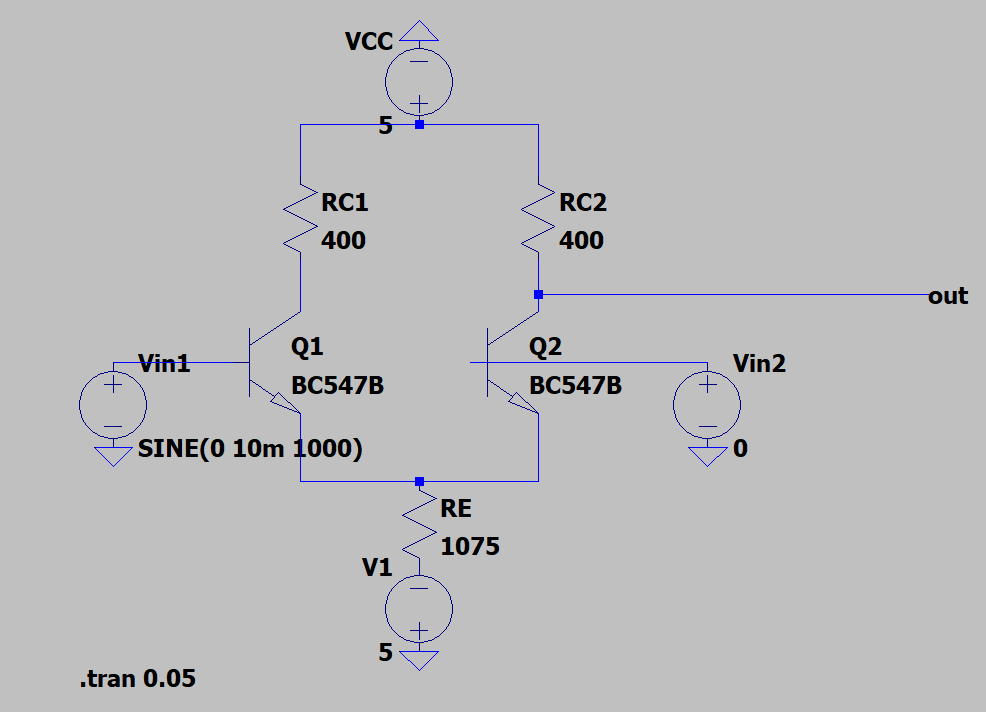
\includegraphics[width=0.85\linewidth]{images/stage1_schematic_ltspice.png}
    \caption{Stage 1 --- LTspice schematic of the differential pre-amplifier.}
    \label{fig:s1_schem}
\end{figure}

\begin{figure}[H]
    \centering
    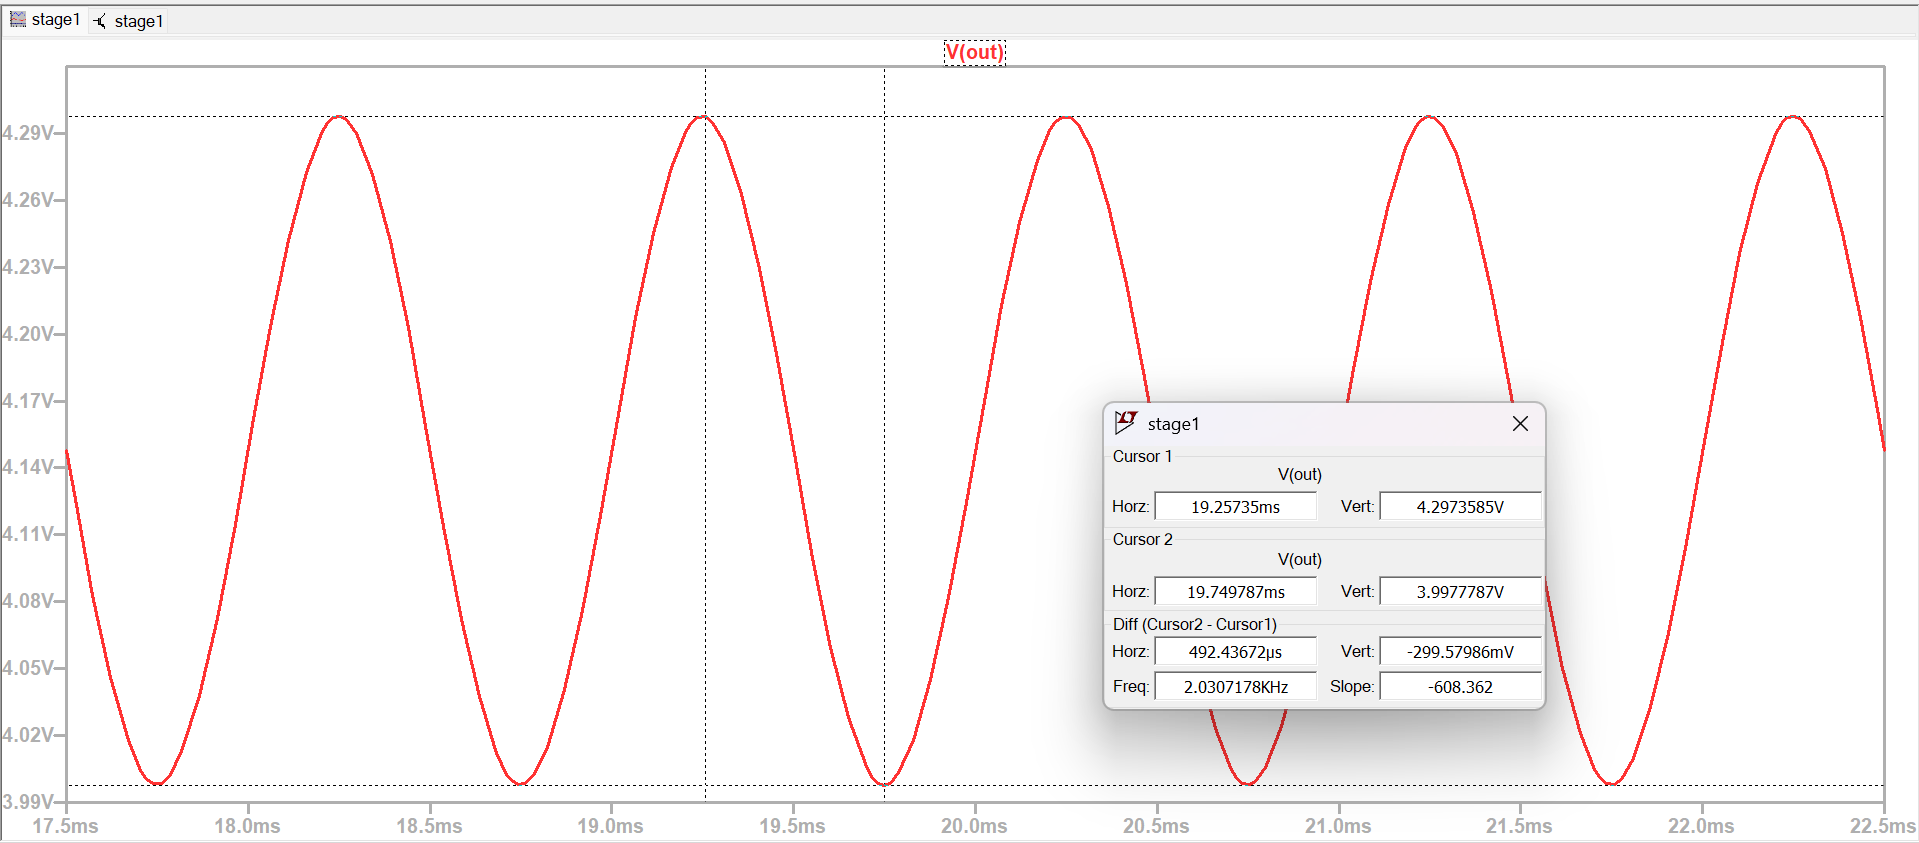
\includegraphics[width=0.85\linewidth]{images/stage1_waveform_ltspice.png}
    \caption{Stage 1 --- LTspice transient waveform showing input (green) and amplified output (blue).}
    \label{fig:s1_wave}
\end{figure}

\begin{figure}[H]
    \centering
    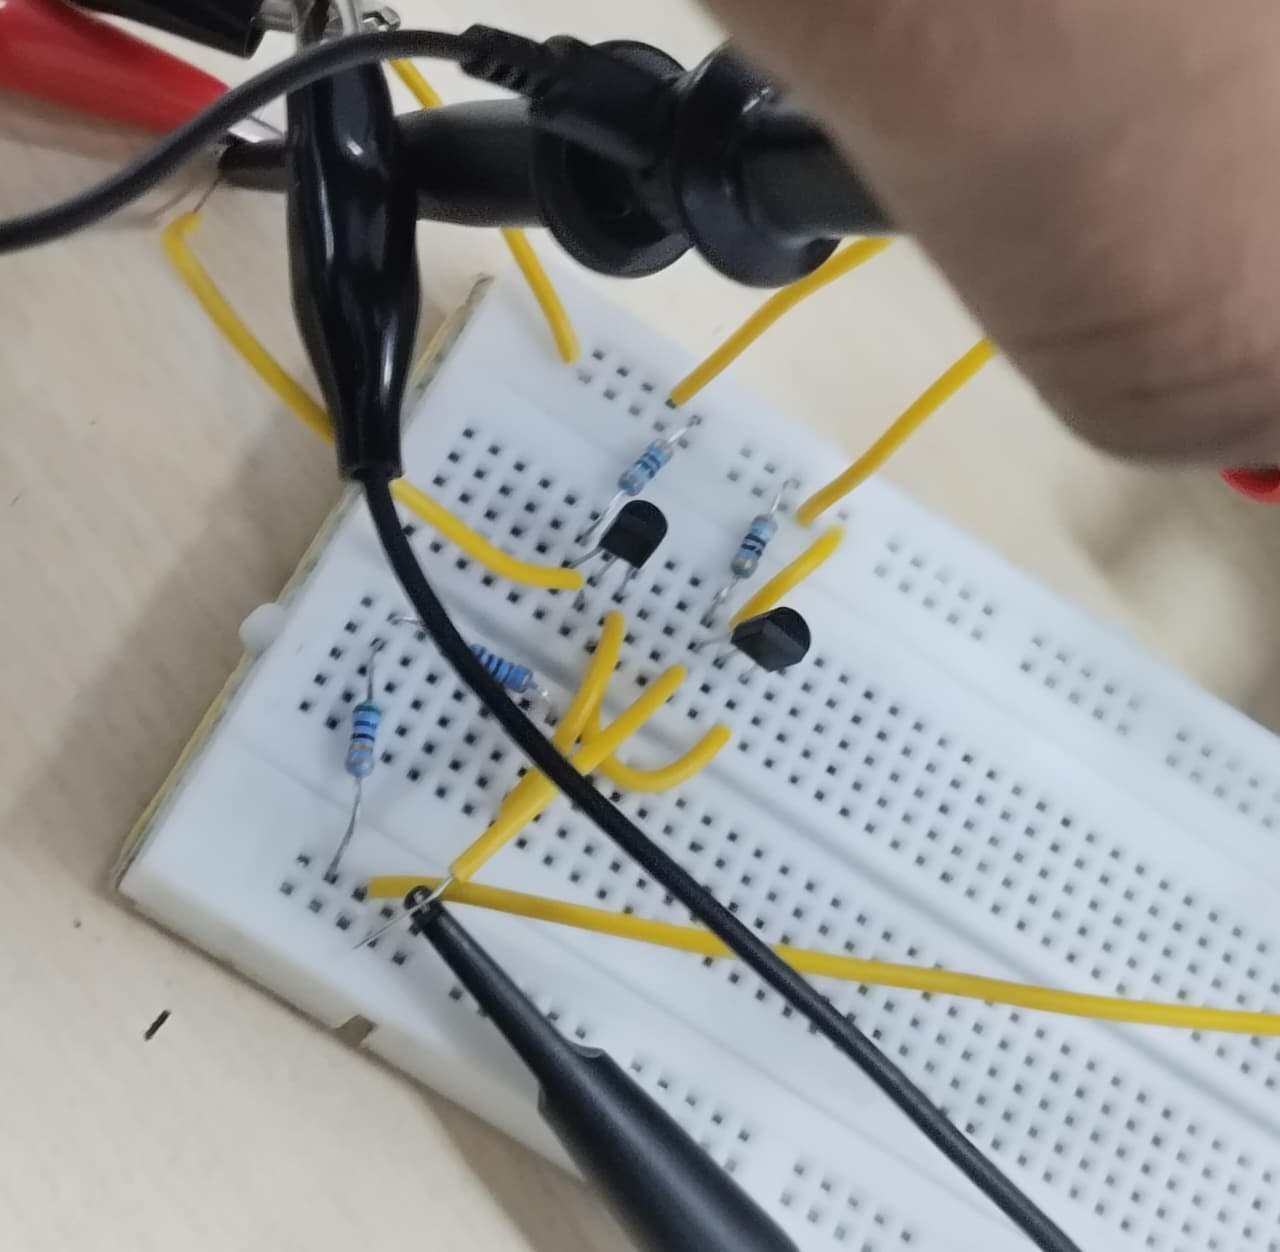
\includegraphics[width=0.85\linewidth]{images/stage1_hw_circuit.png}
    \caption{Stage 1 --- Hardware breadboard implementation.}
    \label{fig:s1_hw}
\end{figure}

\begin{figure}[H]
    \centering
    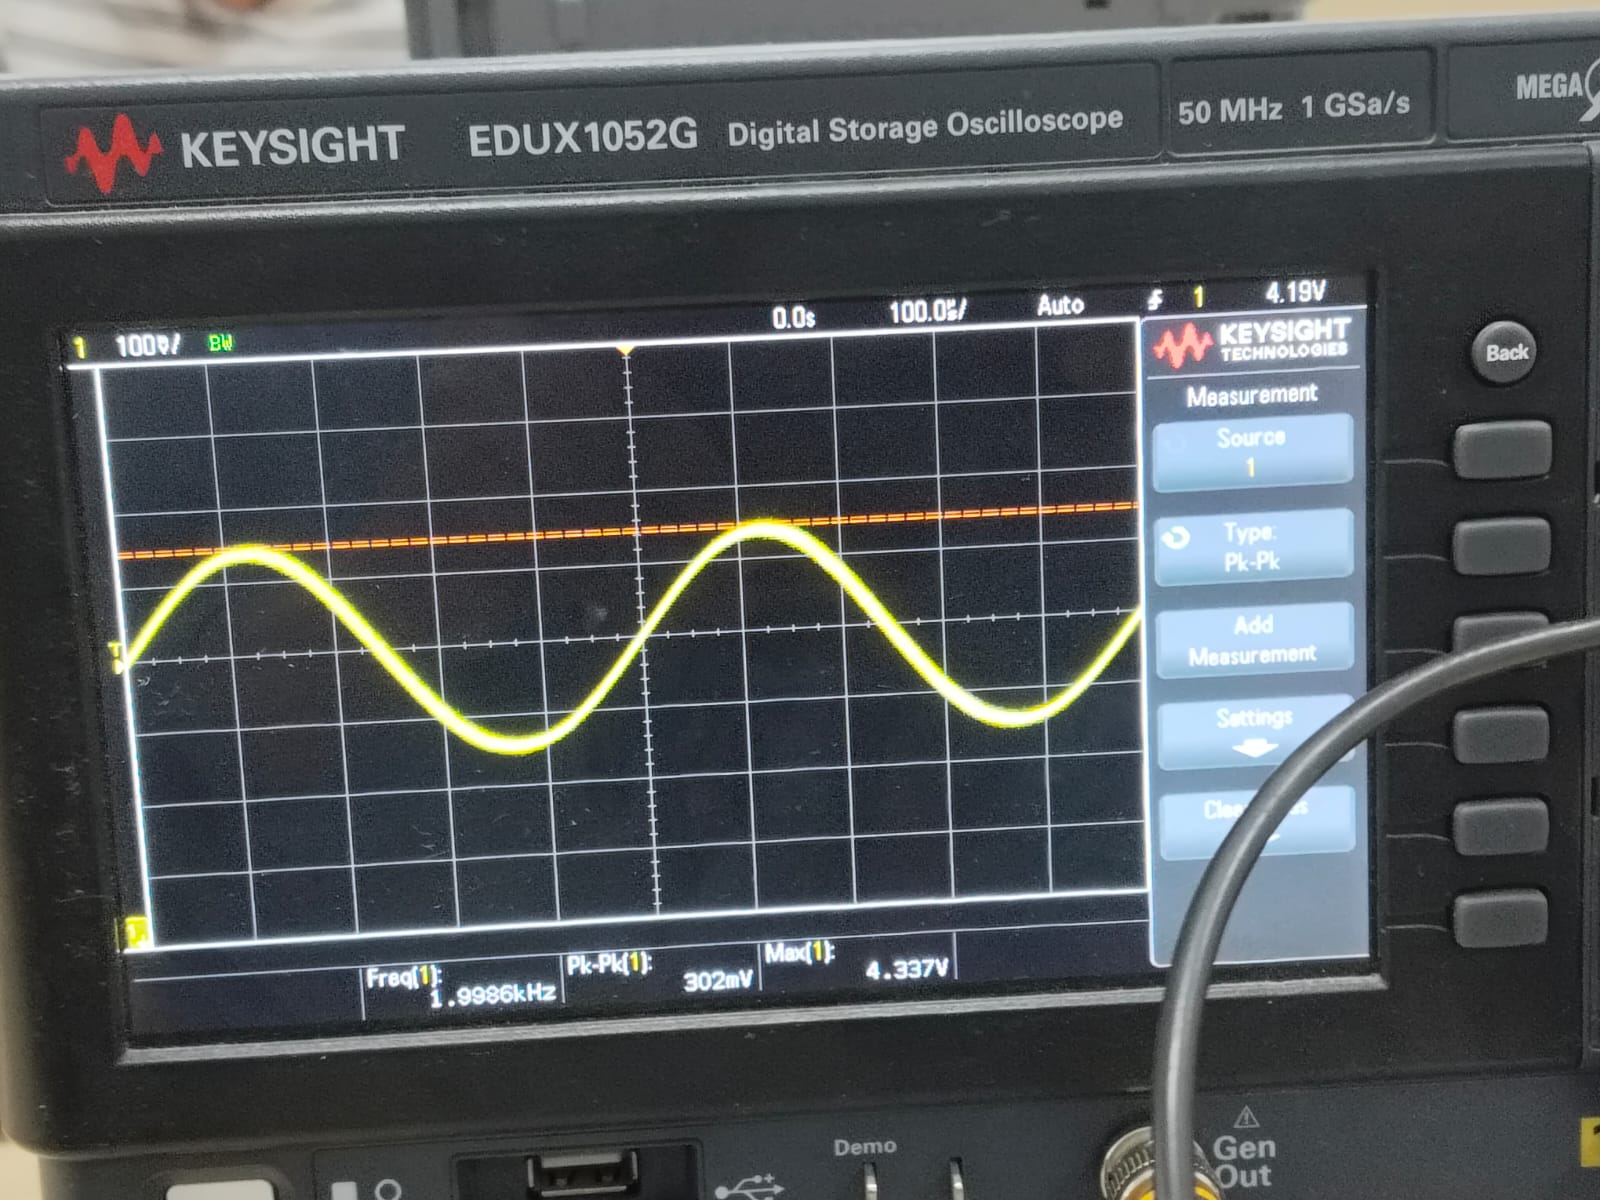
\includegraphics[width=0.85\linewidth]{images/stage1_hw_waveform.png}
    \caption{Stage 1 --- Oscilloscope capture of the hardware output.}
    \label{fig:s1_hw_wave}
\end{figure}

\begin{figure}[H]
    \centering
    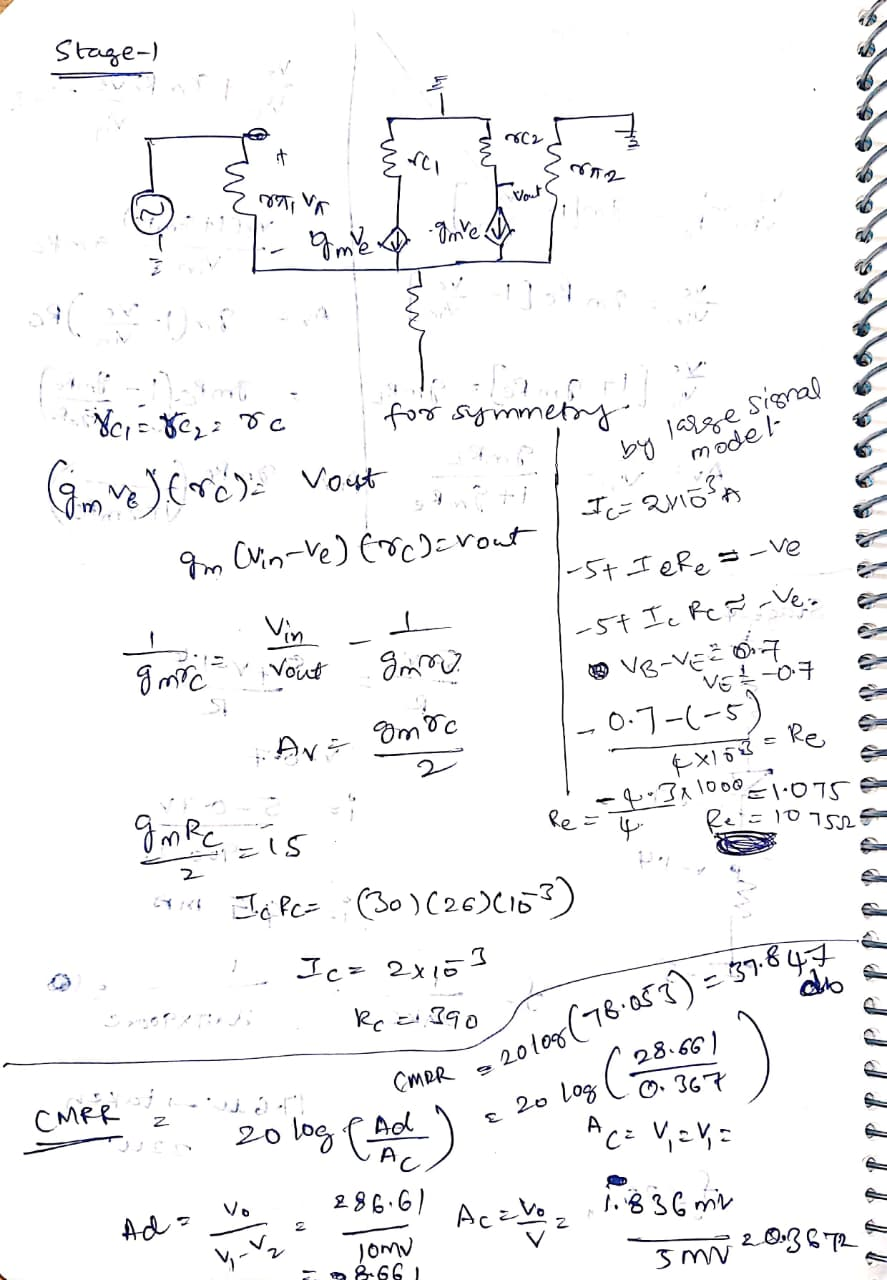
\includegraphics[width=0.85\linewidth]{images/stage1_calculations.png}
    \caption{Stage 1 --- Hand-written gain and bias calculations.}
    \label{fig:s1_calc}
\end{figure}

% ══════════════════════════════════════════════════════════════
\section{Stage 2: Common-Emitter Gain Stage}
% ══════════════════════════════════════════════════════════════

\subsection{Circuit Description}
A \textbf{common-emitter (CE) amplifier} using BC547B ($Q_3$) provides the bulk of the voltage gain. The CE topology is selected for its:
\begin{itemize}[nosep]
    \item High voltage and current gain.
    \item High input impedance (does not load Stage~1).
    \item Low output impedance (drives the filter stage).
\end{itemize}

\subsection{Biasing Design}
\subsection{Common Emitter (CE) Amplifier Biasing}

The CE amplifier is biased using a dual supply of $+5\,V$ and $-5\,V$. 
The desired base bias voltage is set to

\[
V_B = -4.2\,V
\]

\subsubsection*{Voltage Divider Design}

Let $R_{B1}$ be connected to $+5\,V$ and $R_{B2}$ to $-5\,V$.

Using voltage division between $+5\,V$ and $-5\,V$:

\[
V_B = V_{-5} + \frac{R_{B2}}{R_{B1}+R_{B2}} (V_{+5}-V_{-5})
\]

Substituting values:

\[
-4.2 = -5 + \frac{R_{B2}}{R_{B1}+R_{B2}} (10)
\]

\[
0.8 = 10 \frac{R_{B2}}{R_{B1}+R_{B2}}
\]

\[
\frac{R_{B2}}{R_{B1}+R_{B2}} = 0.08
\]

\[
R_{B2} = 0.08 (R_{B1}+R_{B2})
\]

\[
0.92 R_{B2} = 0.08 R_{B1}
\]

\[
R_{B1} = 11.5 R_{B2}
\]

Choosing a practical value:

if \[
R_{B2} = 0.4\,k\Omega
\]

\[
R_{B1} \approx 4.6\,k\Omega
\]


\subsubsection*{Emitter Voltage}

For a silicon BJT,

\[
V_{BE} \approx 0.7\,V
\]

\[
V_E = V_B - V_{BE}
\]

\[
V_E = -4.2 - 0.7
\]

\[
V_E = -4.9\,V
\]

Thus, the emitter is approximately at the negative supply potential.

\subsubsection*{Verification of Active Region Operation}

For an NPN transistor to operate in the active region:

\[
V_C > V_B > V_E
\]

Since:

\[
V_B = -4.2\,V
\]
\[
V_E = -4.9\,V
\]

\[
V_B - V_E = 0.7\,V
\]

The base-emitter junction is forward biased.

If the collector voltage satisfies:

\[
V_C > -4.2\,V
\]

then:
we operate the Vc such that it stops when it is reaching the saturation voltage that iswhen the difference is lesser than 0.2V so for the 20mV peak to peak we get the minimum voltage is around -4.7 which is -4.9+0.2
\[
V_{CE} = V_C - V_E > 0.2\,V
\]

which ensures the transistor operates in the active region.

Hence, the CE amplifier is properly biased in the active region.
(In practice, $I_C$ is lower due to $\beta$ effects; the simulated operating point confirms active-region operation.)

% \paragraph{Stability Factor:}
% \begin{equation}
%     S = \frac{\partial I_C}{\partial I_{CBO}} = \frac{\beta + 1}{1 - \beta\,\dfrac{\partial I_B}{\partial I_C}}
% \end{equation}
% With the voltage-divider bias, $S$ is small, ensuring stable biasing across temperature.

\subsection{Small-Signal Gain}
\begin{equation}
    A_v = \frac{-g_m (R_C \| R_L)}{1 + g_m R_E}
\end{equation}
With $R_C = 2.5\;\text{k}\Omega$, $R_1 = 60\;\Omega$ (emitter degeneration), and the bypass capacitor $C_E = 470\;\mu\text{F}$ shorting $R_E$ at audio frequencies:
\subsection{Gain Calculation}

The required voltage gain for the amplifier is

\[
A_v = 33
\]

For a Common Emitter (CE) amplifier with emitter degeneration, the voltage gain is given by

\[
A_v = \frac{g_m R_C}{1 + g_m R_E}
\]

Substituting the obtained values,
\subsection{Gain Calculation}

The required voltage gain for the amplifier is

\[
A_v = 33
\]

For a Common Emitter (CE) amplifier with emitter degeneration, the voltage gain is given by

\[
A_v = \frac{g_m R_C}{1 + g_m R_E}
\]

The transconductance is

\[
g_m = \frac{I_C}{V_T}
\]

Taking the thermal voltage

\[
V_T \approx 25\,\text{mV}
\]

Given

\[
I_C = 2.1\,\text{mA}
\]

\[
R_C = 2.388\,k\Omega
\]

\[
R_E = 68\,\Omega
\]

Thus,

\[
g_m = \frac{2\,\text{mA}}{25\,\text{mV}}
\]

\[
g_m = \frac{0.002}{0.025}
\]

\[
g_m = 0.084\,\text{S}
\]

Substituting the values,

\[
A_v =
\frac{(0.084)(2388)}
{1 + (0.084)(68)}
\]

\[
A_v =
\frac{230.4}{1 + 5.44}
\]

\[
A_v =
\frac{200.5}{6.44}
\]

\[
A_v \approx 31.2
\]

Thus, the obtained voltage gain is approximately

\[
A_v \approx 31.2
\]

which is close to the required gain of

\[
A_v = 33
\]

Hence, the designed CE amplifier satisfies the gain requirement.

Thus, after substituting the calculated component values, we obtain the final gain as

\[
A_v \approx 33
\]

Hence, the designed CE amplifier successfully achieves the required voltage gain.
The CE stage is designed so that the combined gain of Stages 1 and 2 satisfies $G_1 \times G_2 \sim 500$.

\begin{figure}[H]
    \centering
    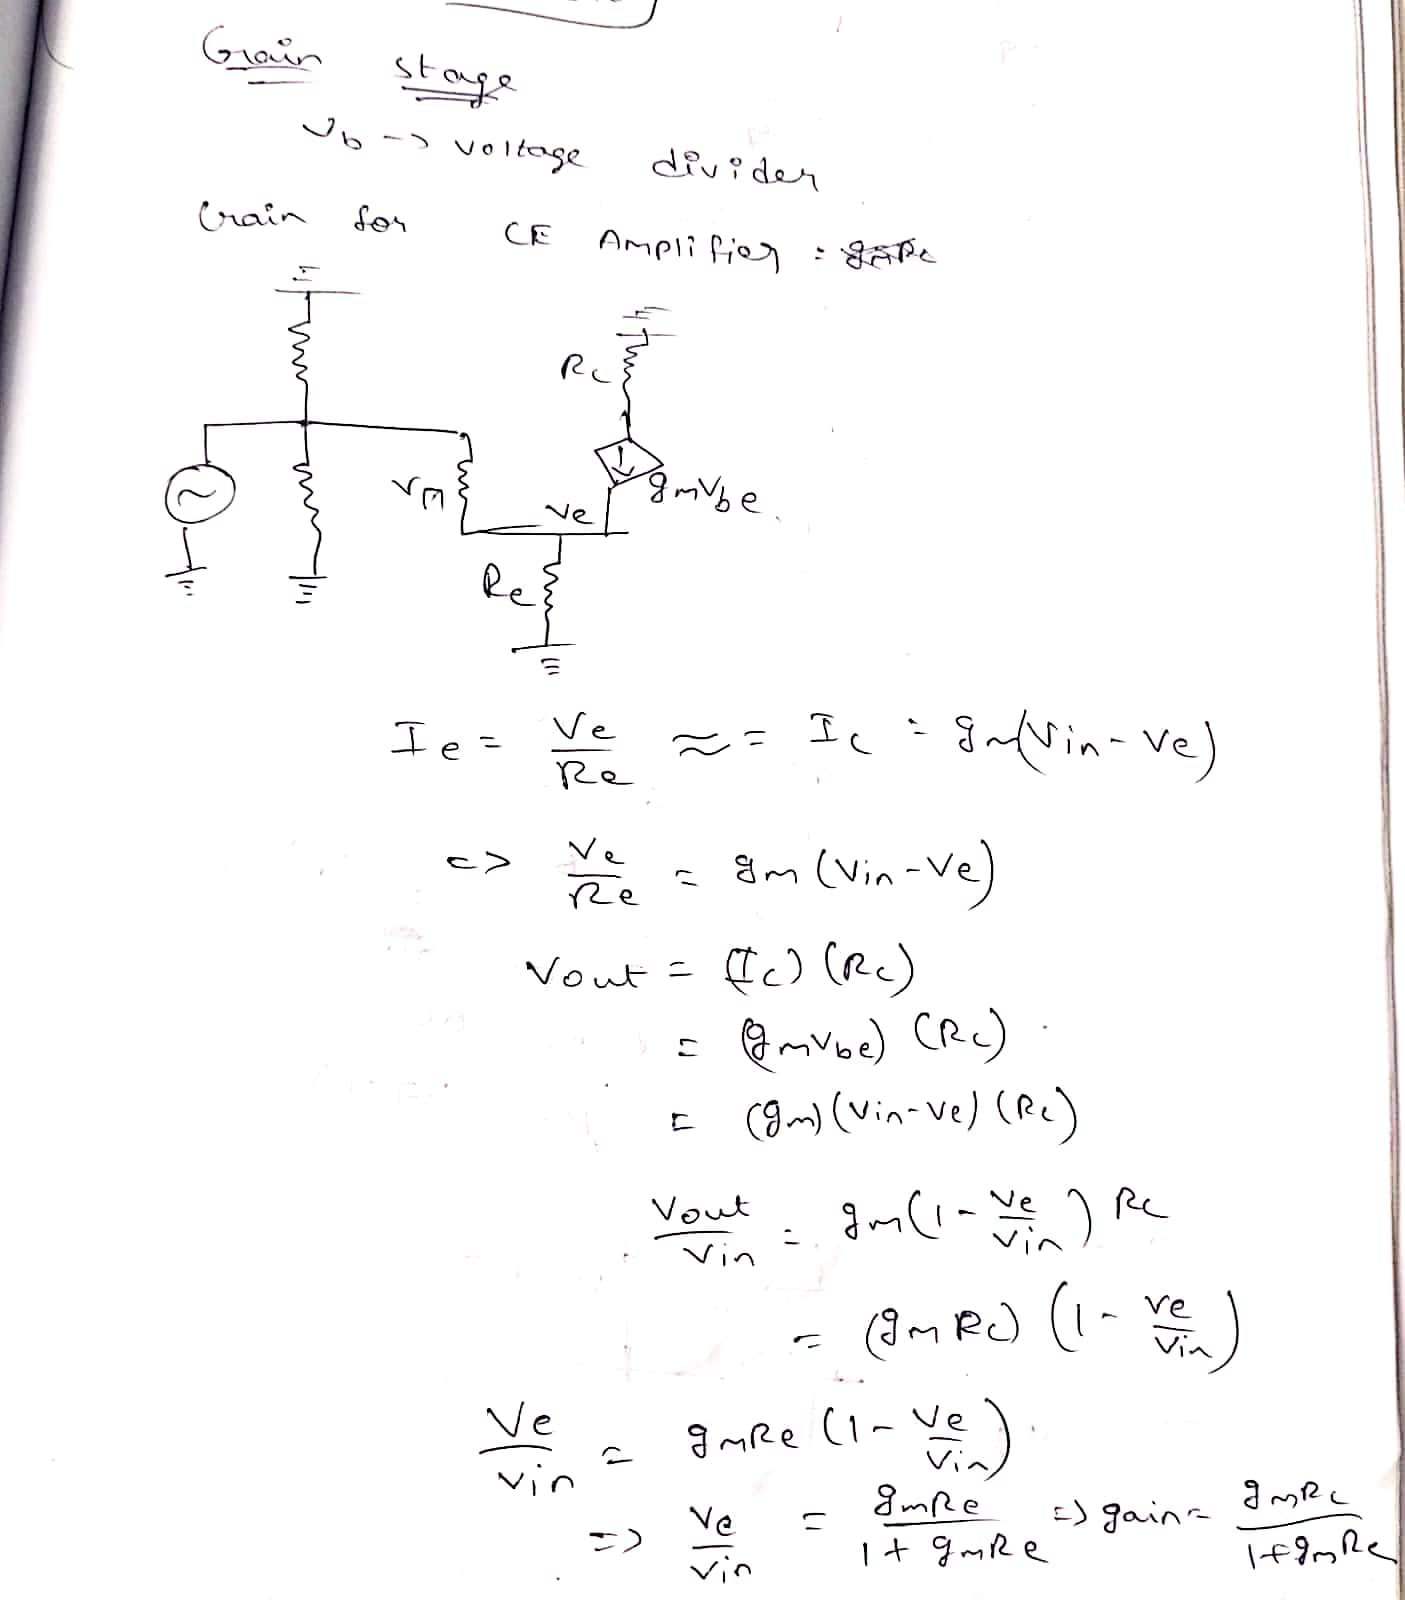
\includegraphics[width=0.85\linewidth]{images/stage2_smallsignal_derivation.png}
    \caption{Stage 2 --- Hand-written small-signal analysis and voltage gain derivation.}
    \label{fig:s2_ss_deriv}
\end{figure}

\begin{figure}[H]
    \centering
    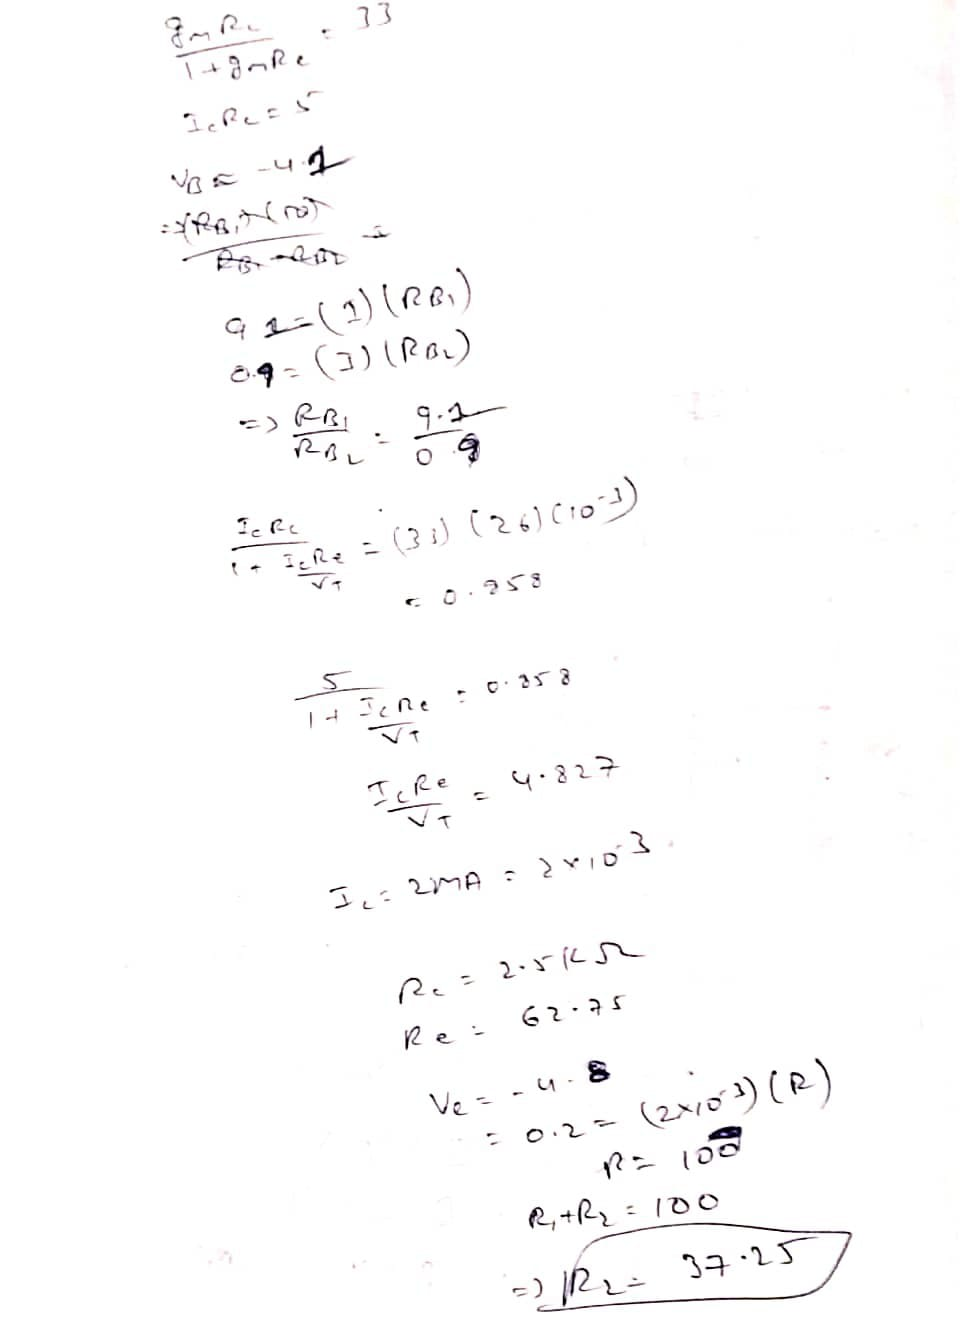
\includegraphics[width=0.85\linewidth]{images/stage2_value_calculations.png}
    \caption{Stage 2 --- Hand-written component value calculations for biasing and gain.}
    \label{fig:s2_val_calc}
\end{figure}

\subsection{AC Coupling}
\begin{itemize}[nosep]
    \item $C_1 = 470\;\mu\text{F}$ — input coupling capacitor; blocks DC from Stage~1. Its impedance at $20\;\text{Hz}$: $X_{C1} = 1/(2\pi \cdot 20 \cdot 470\times10^{-6}) \approx 16.9\;\Omega$, which is much less than $R_{in}$, so low-frequency content passes.
    \item $C_E = 470\;\mu\text{F}$ — emitter bypass; shorts $R_E$ at AC frequencies, boosting gain.
    \item $C_2 = 470\;\mu\text{F}$ — output coupling capacitor; blocks DC to the filter stage.
\end{itemize}

\subsection{LTspice Circuit and Waveforms}

\begin{figure}[H]
    \centering
    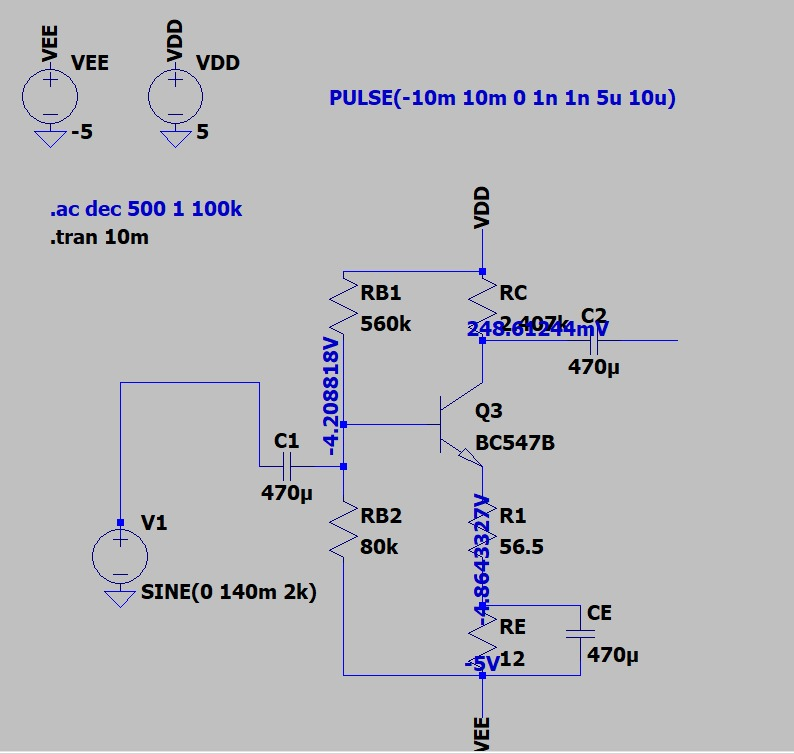
\includegraphics[width=0.85\linewidth]{images/stage2_ltspice_circuit.png}
    \caption{Stage 2 --- LTspice schematic of the common-emitter gain stage.}
    \label{fig:s2_schem}
\end{figure}

\begin{figure}[H]
    \centering
    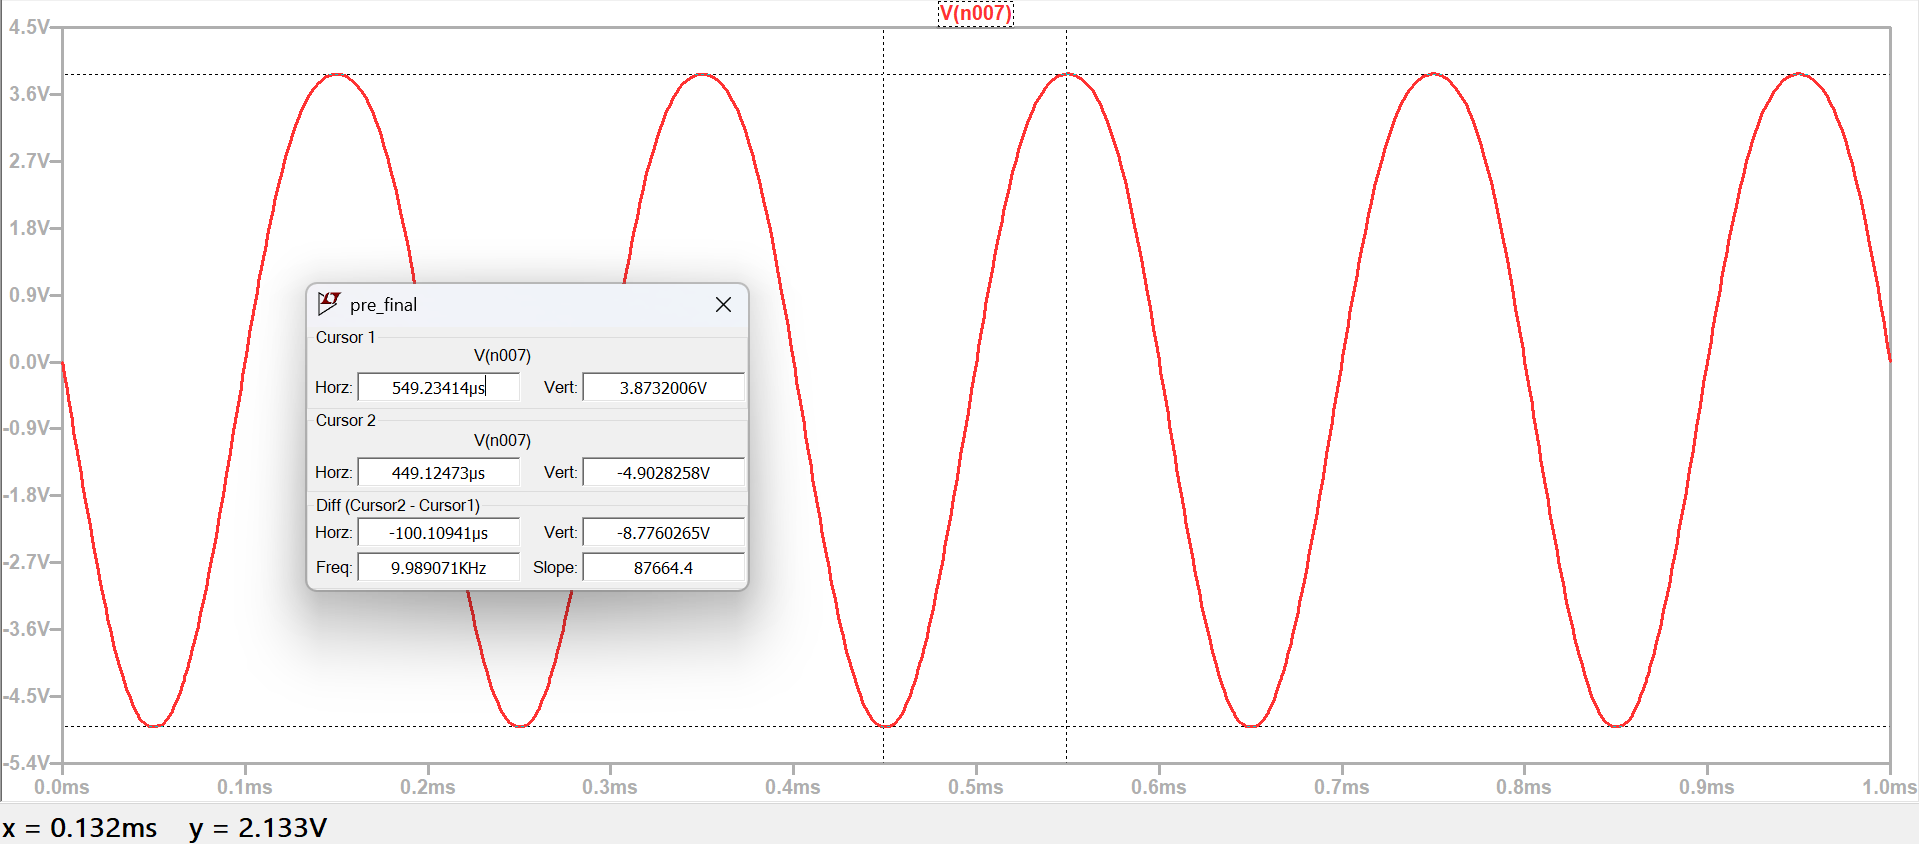
\includegraphics[width=0.85\linewidth]{images/stage2_waveform_ltspice.png}
    \caption{Stages 1+2 --- LTspice transient waveform showing amplified output after the CE stage.}
    \label{fig:s2_wave}
\end{figure}

% \begin{figure}[H]
%     \centering
%     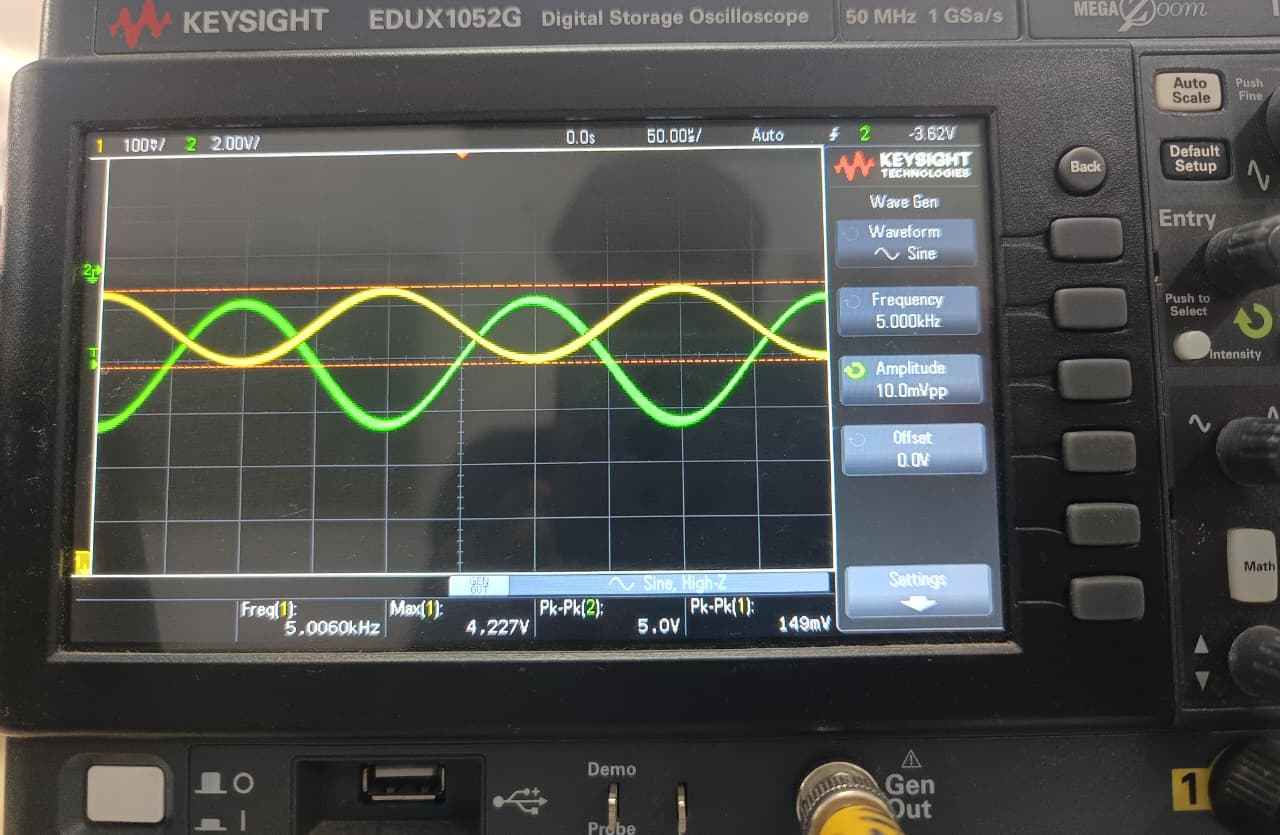
\includegraphics[width=0.85\linewidth]{images/stage2_hw_waveform.png}
%     \caption{Stage 2 --- Oscilloscope capture of the hardware output after the CE gain stage ($150\;\text{mV}_{pp}$ or $300\;\text{mV}_{pp}$ input).}
%     \label{fig:s2_hw_wave}
% \end{figure}

After integrating the first and the second circuit we have seen that the impedance had affected because the initial resistances are lesser which will affect the output impedance of the first circuit which tends to decrease the amplification due to the first stage.
But when we increase the resistances for the biasing circuit the current flowing through the branch will become very less which will be easily affected by the small changes flowing out of the capacitor, so we have increased the resistances and the ratio of the biasing resistances.
The total voltage gain obtained after cascading the two stages is approximately $450$ for a $20\;\text{mV}_{pp}$ input signal. When the input amplitude is reduced to $10\;\text{mV}_{pp}$, the overall gain increases to $500$, which matches the expected theoretical gain of the design.

Now we have two resistances at the emitter of the BJT --- one is for maintaining the bias voltage and the other for maintaining the voltage gain. The maintaining of the bias voltage is required because the voltage gain we require is around $500$ and the maximum input is at $20\;\text{mV}$, which results in exactly $+5\;\text{V}$ to $-5\;\text{V}$, so we will keep the bias voltage to be zero for not making it clip.

\subsection{Hardware Results (Stage 1 + Stage 2)}

\begin{figure}[H]
    \centering
    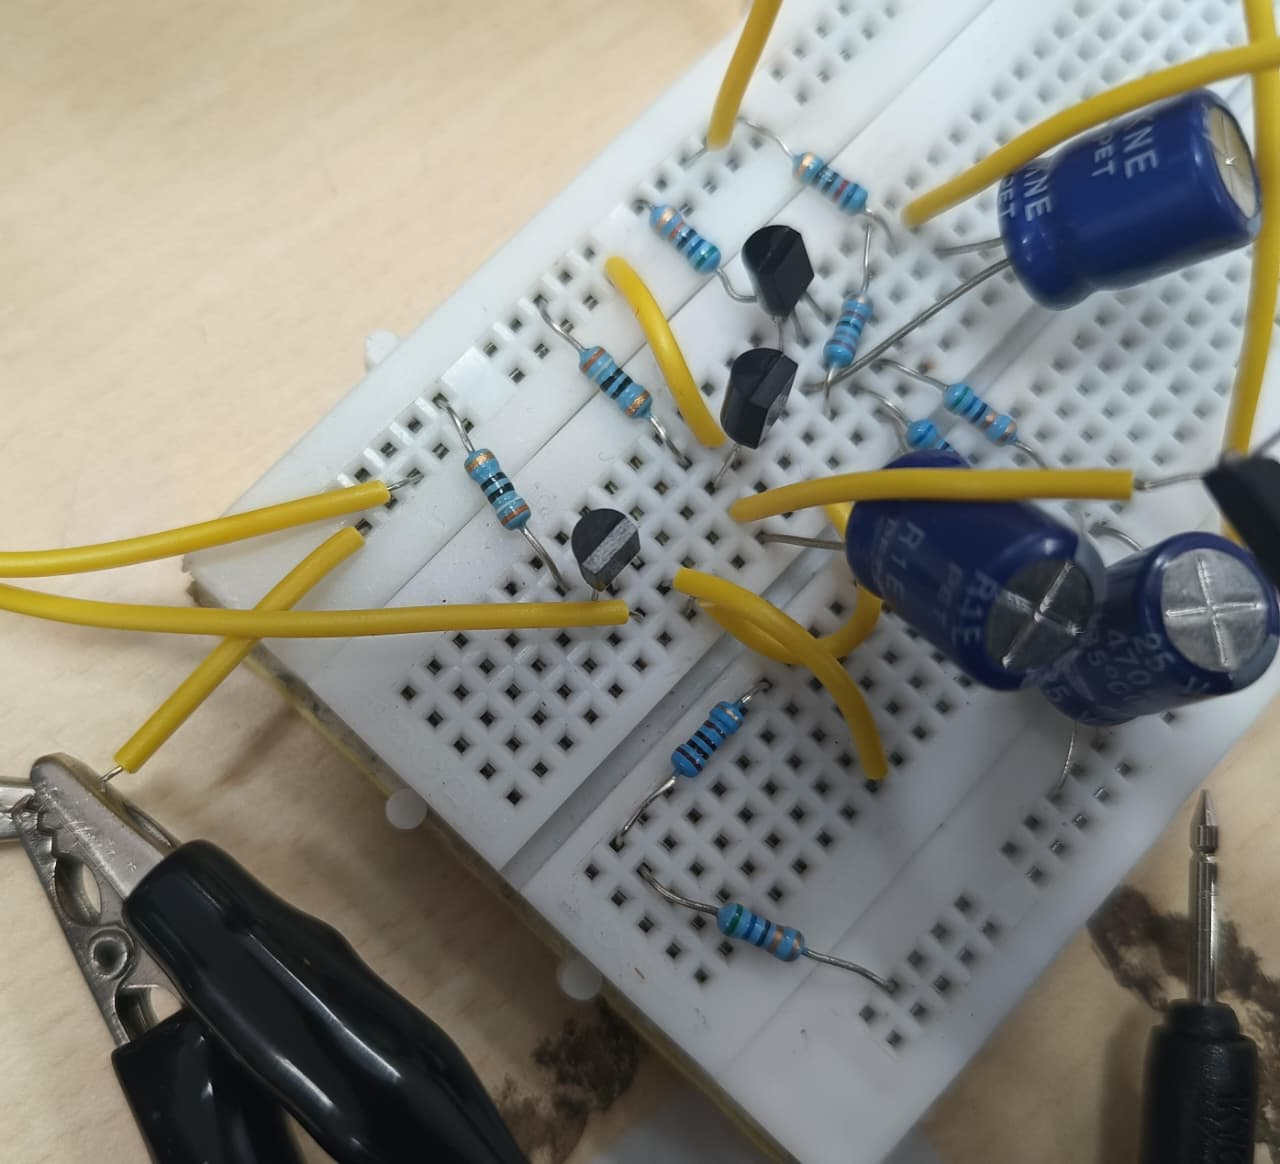
\includegraphics[width=0.85\linewidth]{images/stage2_hw_circuit.png}
    \caption{Stages 1+2 --- Hardware breadboard implementation of the differential pre-amplifier and CE gain stage.}
    \label{fig:s2_hw_circuit}
\end{figure}

\begin{figure}[H]
    \centering
    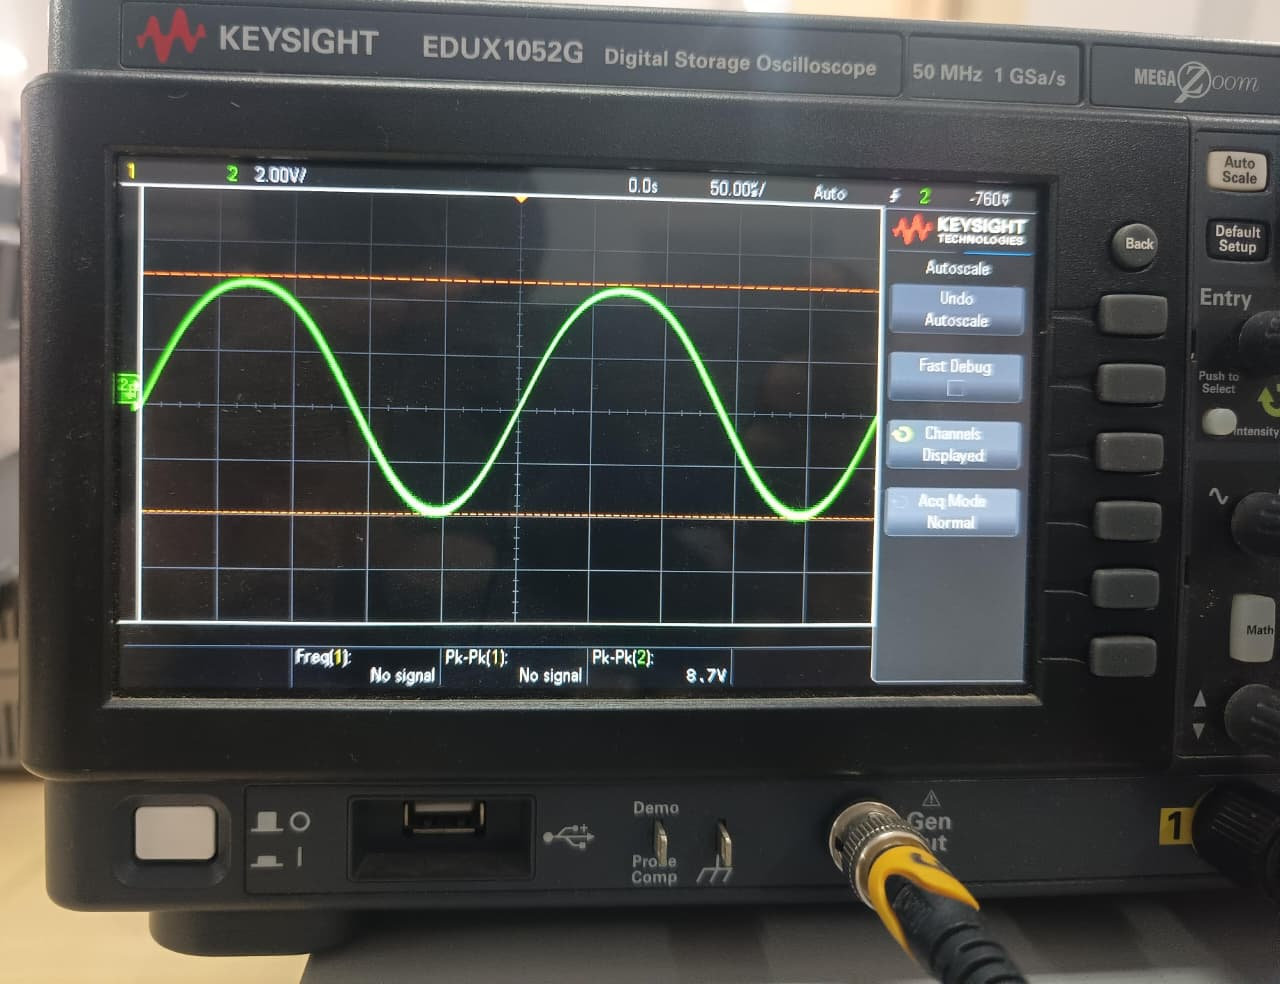
\includegraphics[width=0.85\linewidth]{images/stage2_hw_waveform_20mv.png}
    \caption{Stages 1+2 --- Oscilloscope output for $20\;\text{mV}_{pp}$ input. Overall gain $\approx 435$.}
    \label{fig:s2_hw_wave_20mv}
\end{figure}

\begin{figure}[H]
    \centering
    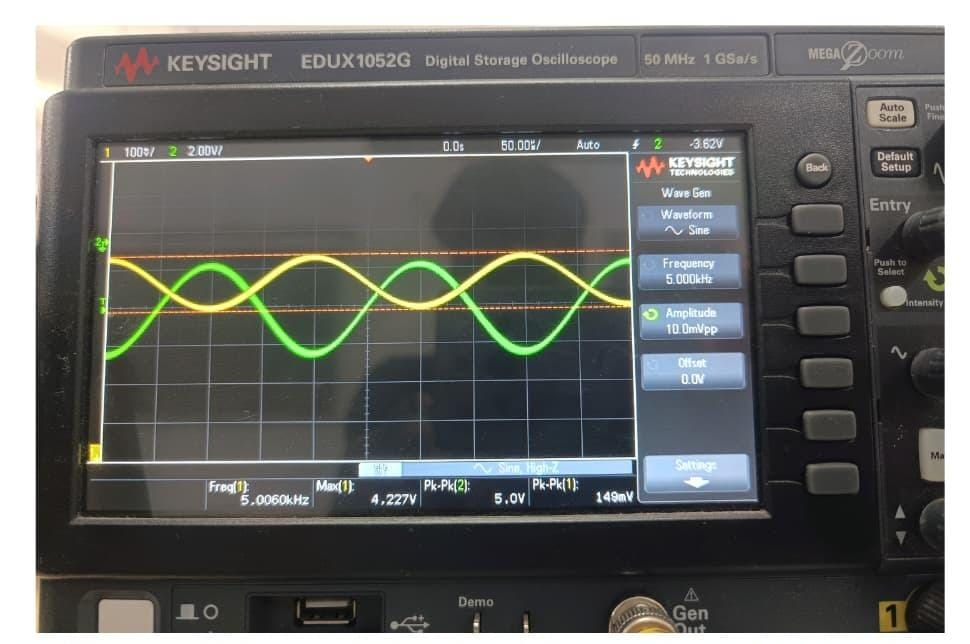
\includegraphics[width=0.85\linewidth]{images/stage2_hw_waveform_10mv.png}
    \caption{Stages 1+2 --- Oscilloscope output for $10\;\text{mV}_{pp}$ input. Overall gain $\approx 500$, matching the theoretical design target.}
    \label{fig:s2_hw_wave_10mv}
\end{figure}

% ══════════════════════════════════════════════════════════════
\section{Stage 3: Band-Pass Filter (20\,Hz -- 20\,kHz)}
% ══════════════════════════════════════════════════════════════

\subsection{Purpose}
This stage limits the signal to the audible range ($20\;\text{Hz}$--$20\;\text{kHz}$).
Frequencies outside this range carry no useful audio and can cause distortion in the power stage.

\subsection{Implementation}
An \textbf{active BPF} is built by combining a high-pass and a low-pass RC network around a
\textbf{UA741 op-amp}. Active filters are used because:
\begin{itemize}[nosep]
    \item Unity passband gain can be maintained without attenuation.
    \item The op-amp buffers the signal, so the filter does not load Stage~2.
    \item Better stability compared to a passive RC design.
\end{itemize}

\begin{figure}[H]
    \centering
    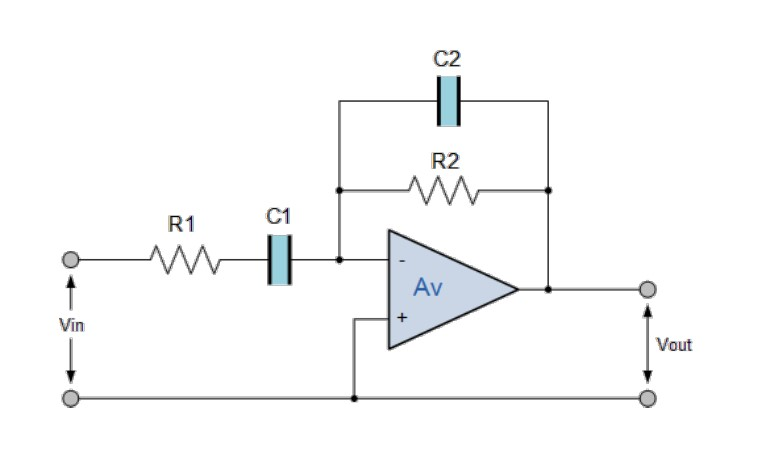
\includegraphics[width=0.9\linewidth]{images/active-bpf.png}
    \caption{Stage 3 --- Active BPF schematic (UA741, inverting configuration).}
    \label{fig:s3_schematic}
\end{figure}

\subsection{Circuit Description}
The UA741 is in the \textbf{inverting} configuration. Two RC networks set the frequency response.

\paragraph{Input network ($R_1$, $C_1$) — High-pass:}
At low frequencies $C_1$ is nearly open, blocking the signal.
At high frequencies $C_1$ is nearly short, letting the signal through.
Cutoff: $f_L = 1/(2\pi R_1 C_1)$.

\paragraph{Feedback network ($R_2$, $C_2$) — Low-pass:}
At low frequencies $C_2$ is open so feedback is just $R_2$.
At high frequencies $C_2$ shorts $R_2$, increasing negative feedback and attenuating the signal.
Cutoff: $f_H = 1/(2\pi R_2 C_2)$.

So low frequencies are blocked at the input and high frequencies are killed by the feedback — giving the band-pass response.

\subsection{Why Inverting Configuration?}

\paragraph{Not non-inverting:}
Non-inverting gain is $A_v = 1 + R_2/R_1$. For unity gain we need $R_2/R_1 \to 0$,
meaning $R_2$ near zero or $R_1$ near infinity — not practical at all.

\paragraph{Inverting:}
Inverting gain is $A_v = -R_2/R_1$. Simply set $R_1 = R_2$ and $|A_v| = 1$.
Easy to achieve with standard resistors.

\paragraph{Phase bonus:}
The inverting stage adds $180^{\circ}$ phase shift. Stage~2 (CE) already inverted the signal.
Two inversions = original polarity restored at the filter output.

\subsection{Why $R = 2.2\;\text{M}\Omega$?}
$R_1$ of the BPF sits in parallel with Stage~2's collector load ($\sim 2.5\;\text{k}\Omega$).
A small $R_1$ would reduce that parallel load and hurt Stage~2's gain.
At $2.2\;\text{M}\Omega \gg 2.5\;\text{k}\Omega$, the parallel combination is almost the same
as the Stage~2 load alone — so Stage~2 gain is unaffected.

\subsection{AC Response Derivation}

\begin{equation}
    Z_{in} = R_1 + \frac{1}{j\omega C_1}
\end{equation}
\begin{equation}
    Z_{out} = R_2 \;\Big\Vert\; \frac{1}{j\omega C_2}
            = \frac{R_2}{1 + j\omega R_2 C_2}
\end{equation}

Inverting gain: $A_v = -Z_{out}/Z_{in}$, which gives:

\begin{equation}
    \boxed{A_v(\omega) = -\frac{j\omega R_2 C_1}{\left(1+j\omega R_1 C_1\right)
    \left(1+j\omega R_2 C_2\right)}}
    \label{eq:bpf_tf}
\end{equation}


Magnitude:
\begin{equation}
    |A_v(\omega)| = \frac{\omega R_2 C_1}
    {\sqrt{1+(\omega R_1 C_1)^2}\;\sqrt{1+(\omega R_2 C_2)^2}}
\end{equation}
\subsection{Band Pass Behaviour}

The transfer function of the circuit is

\begin{equation}
A_v(\omega) =
-\frac{j\omega R_2 C_1}
{(1+j\omega R_1 C_1)(1+j\omega R_2 C_2)}
\end{equation}

The impedance of a capacitor is

\[
Z_C = \frac{1}{j\omega C}
\]

\textbf{Low frequency:}

\[
\omega \rightarrow 0
\]

\[
Z_{C_1}, Z_{C_2} \rightarrow \infty
\]

Both capacitors behave as open circuits and

\[
A_v(\omega) \rightarrow 0
\]

Thus no signal passes.

\textbf{High frequency:}

\[
\omega \rightarrow \infty
\]

\[
Z_{C_1}, Z_{C_2} \rightarrow 0
\]

Both capacitors behave as short circuits and the gain again approaches zero.

\textbf{Mid frequencies:}

For frequencies between the two cutoff points,

\[
C_1 \approx 0 \quad (\text{short})
\]

\[
C_2 \approx \infty \quad (\text{open})
\]

Thus the signal passes only when one capacitor behaves as a short circuit and the other behaves as an open circuit, giving the band-pass characteristic.

\paragraph{Mid-band simplification to $-R_2/R_1$:}
In the mid-band ($f_L \ll f \ll f_H$):

\begin{itemize}[nosep]
    \item $C_1$ acts as a short circuit, so $1/(j\omega C_1) = 0$,
          giving $Z_{in} = R_1 + 0 = R_1$.
    \item $C_2$ acts as an open circuit, so $1/(j\omega C_2) = \infty$,
          giving $Z_{out} = R_2 \| \infty = R_2$.
\end{itemize}

Substituting into $A_v = -Z_{out}/Z_{in}$:
\begin{equation}
    A_v\Big|_{\text{mid}} = -\frac{R_2}{R_1}
\end{equation}

The capacitors drop out entirely, leaving a pure resistor ratio independent of frequency.

\begin{figure}[H]
    \centering
    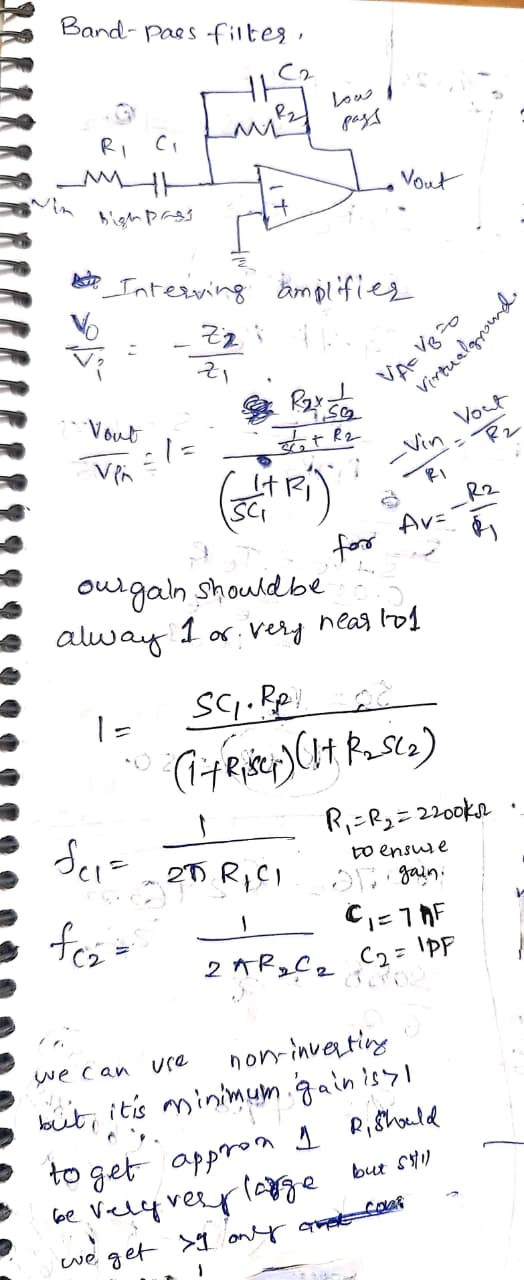
\includegraphics[width=0.9\linewidth]{images/stage3_derivation.png}
    \caption{Stage 3 --- Hand-written AC response derivation.}
    \label{fig:s3_deriv}
\end{figure}

\subsection{Cutoff Frequency Calculations}
$R_1 = R_2 = R = 2.2\;\text{M}\Omega$.

\paragraph{Lower cutoff ($f_L$):}
\begin{equation}
    f_L = \frac{1}{2\pi R_1 C_1}
        = \frac{1}{2\pi \times 2.2\times10^{6} \times 7.33\times10^{-9}}
        \approx 9.83\;\text{Hz}
\end{equation}

\paragraph{Upper cutoff ($f_H$):}
\begin{equation}
    f_H = \frac{1}{2\pi R_2 C_2}
        = \frac{1}{2\pi \times 2.2\times10^{6} \times 1.1\times10^{-12}}
        \approx 65.74\;\text{kHz}
\end{equation}

Both are outside the audio band with some margin for parasitic effects.

\subsection{Mid-Band Gain}
For $f_L \ll f \ll f_H$: $C_1 \approx$ short, $C_2 \approx$ open, so:
\begin{equation}
    A_v = -\frac{R_2}{R_1} = -\frac{2.2\,\text{M}}{2.2\,\text{M}} = -1
    \quad\Longrightarrow\quad |A_v| = 1 \;\;(0\;\text{dB})
\end{equation}

The filter passes the audio signal unchanged in amplitude — exactly as required.

\subsection{Simulation and Hardware Results}
The UA741 runs on $\pm 12\;\text{V}$ rails.

\begin{figure}[H]
    \centering
    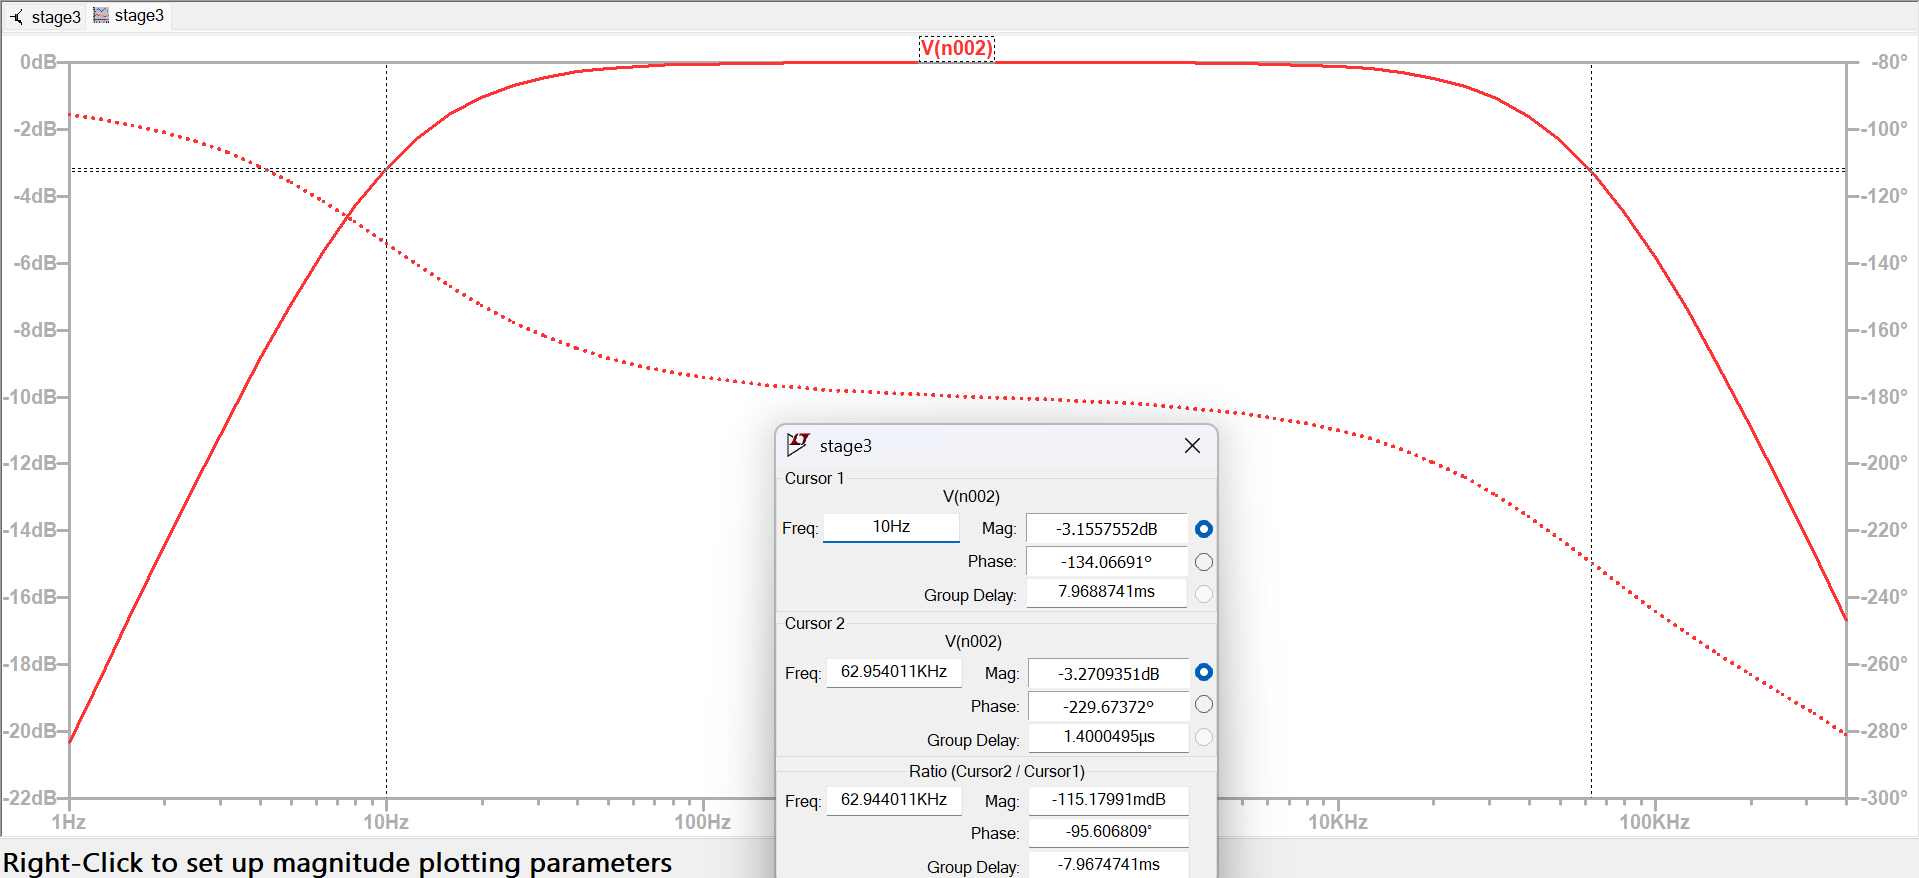
\includegraphics[width=0.85\linewidth]{images/stage3_bode.png}
    \caption{Stage 3 --- LTspice AC Bode plot of the active BPF\@.  The $0\;\text{dB}$
             reference line runs through the middle of the plot; the passband gain is flat
             at $0\;\text{dB}$ between $20\;\text{Hz}$ and $20\;\text{kHz}$, confirming
             unity-gain operation.}
    \label{fig:s3_bode}
\end{figure}

\begin{figure}[H]
    \centering
    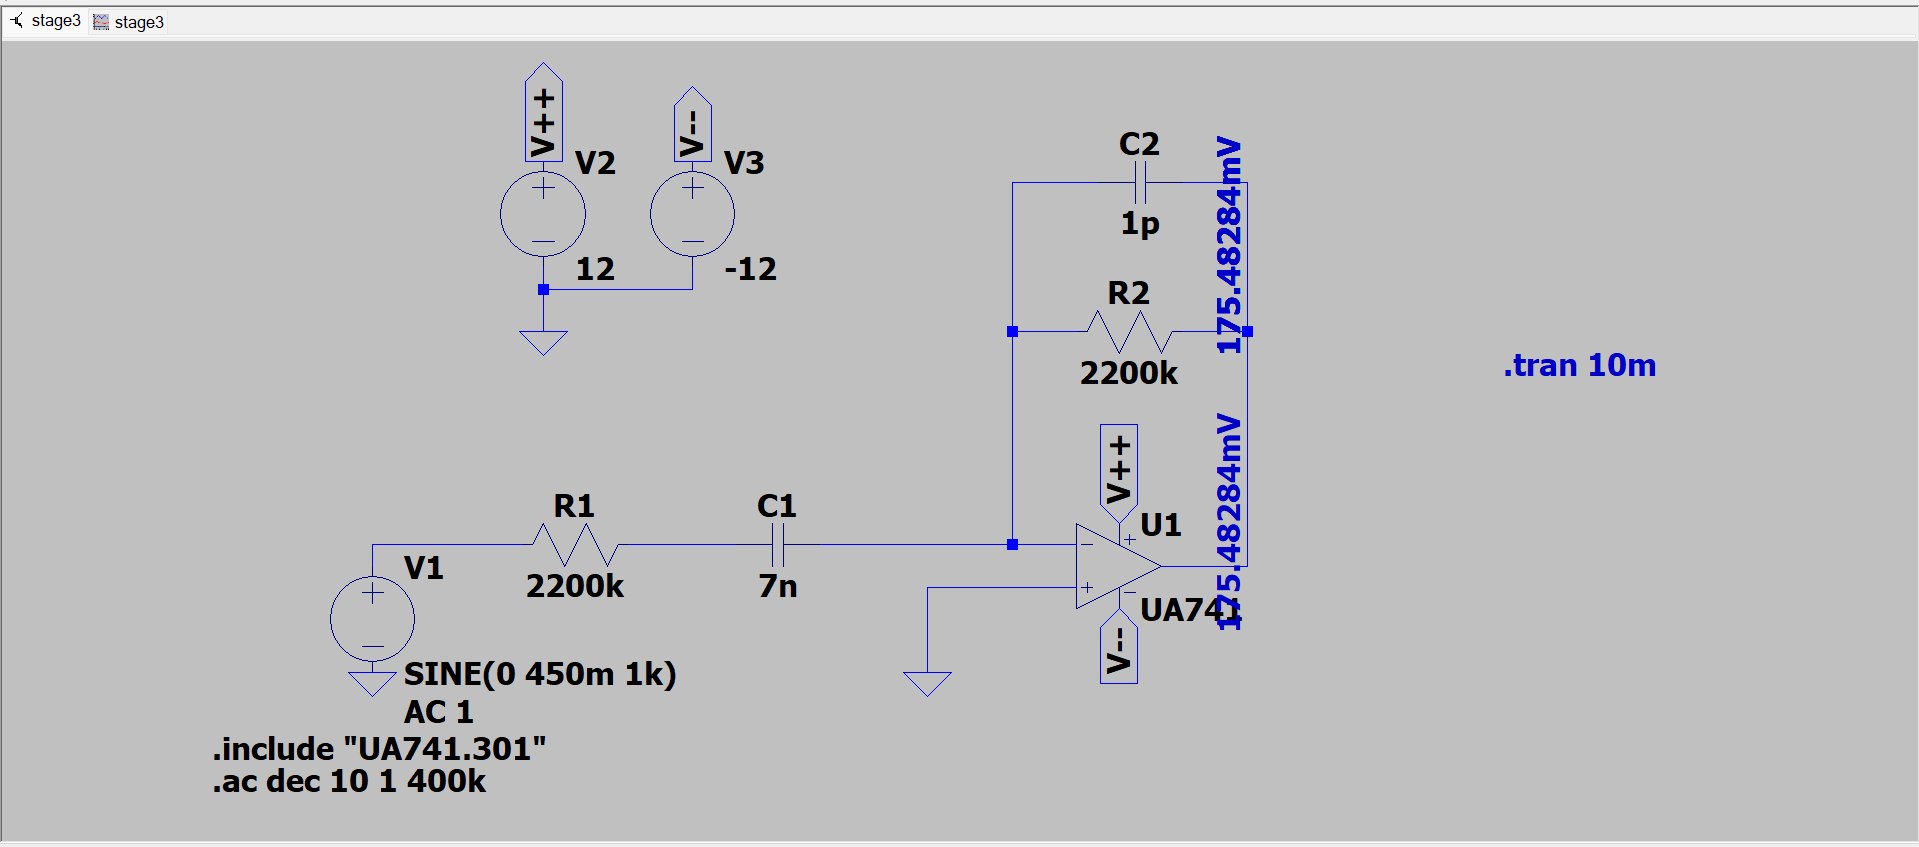
\includegraphics[width=0.85\linewidth]{images/stage3_ltspice_circuit.png}
    \caption{Stage 3 --- LTspice schematic of the active band-pass filter.}
    \label{fig:s3_LT_Spice_circuit}
\end{figure}

\begin{figure}[H]
    \centering
    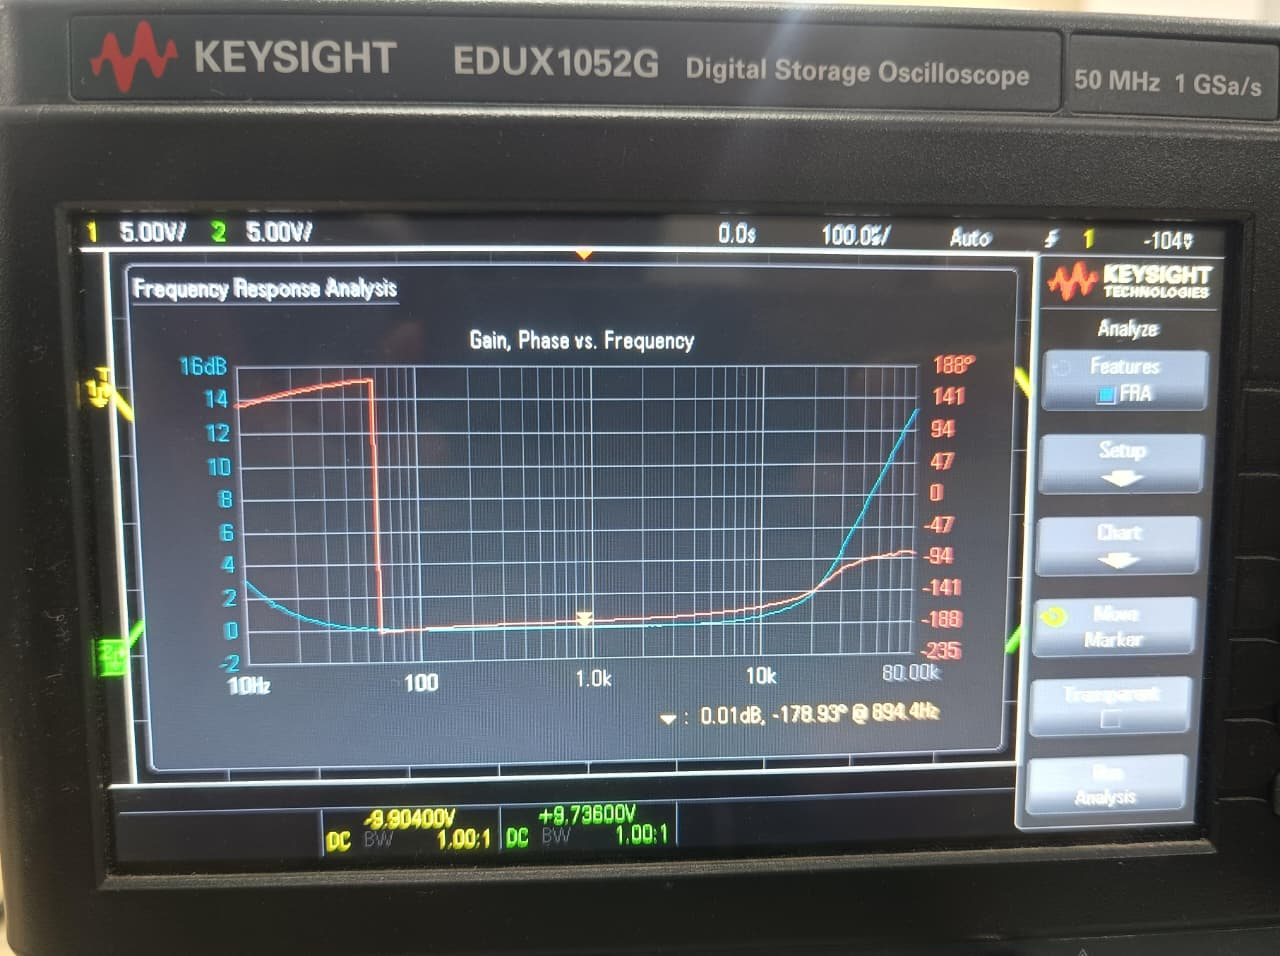
\includegraphics[width=0.85\linewidth]{images/stage3_hw_bode.png}
    \caption{Stage 3 --- Hardware Bode plot.  The $0\;\text{dB}$ line is visible in the
             middle of the plot; the measured passband gain is flat at $0\;\text{dB}$
             across the $20\;\text{Hz}$--$20\;\text{kHz}$ audio band.}
    \label{fig:s3_hw_bode}
\end{figure}
the above bode plot is by mistakenly plotted for V(in)/V(out) because of which the bode plot got reversed


\begin{figure}[H]
    \centering
    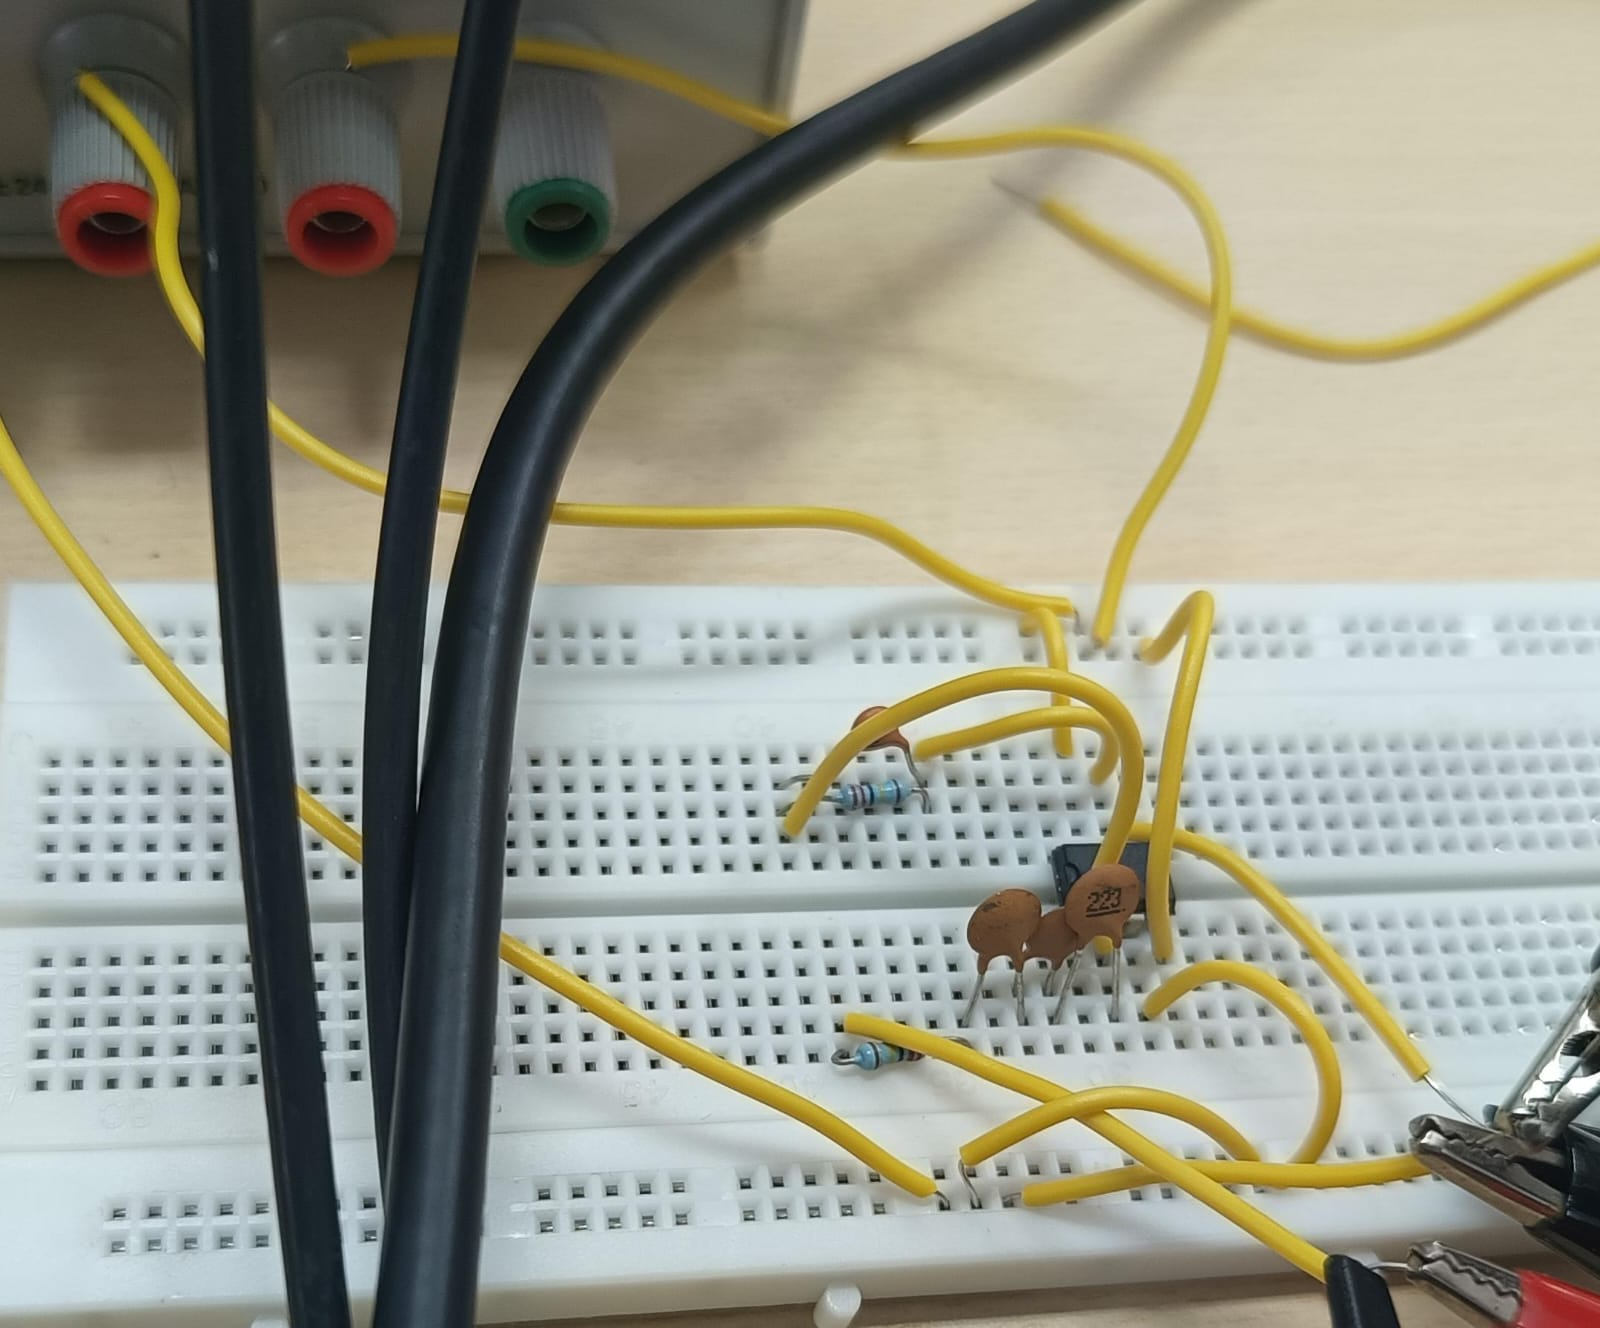
\includegraphics[width=0.85\linewidth]{images/stage3_hw_circuit.png}
    \caption{Stage 3 --- Assembled hardware circuit of the active band-pass filter on
             breadboard.}
    \label{fig:s3_hw_circuit}
\end{figure}

\begin{figure}[H]
    \centering
    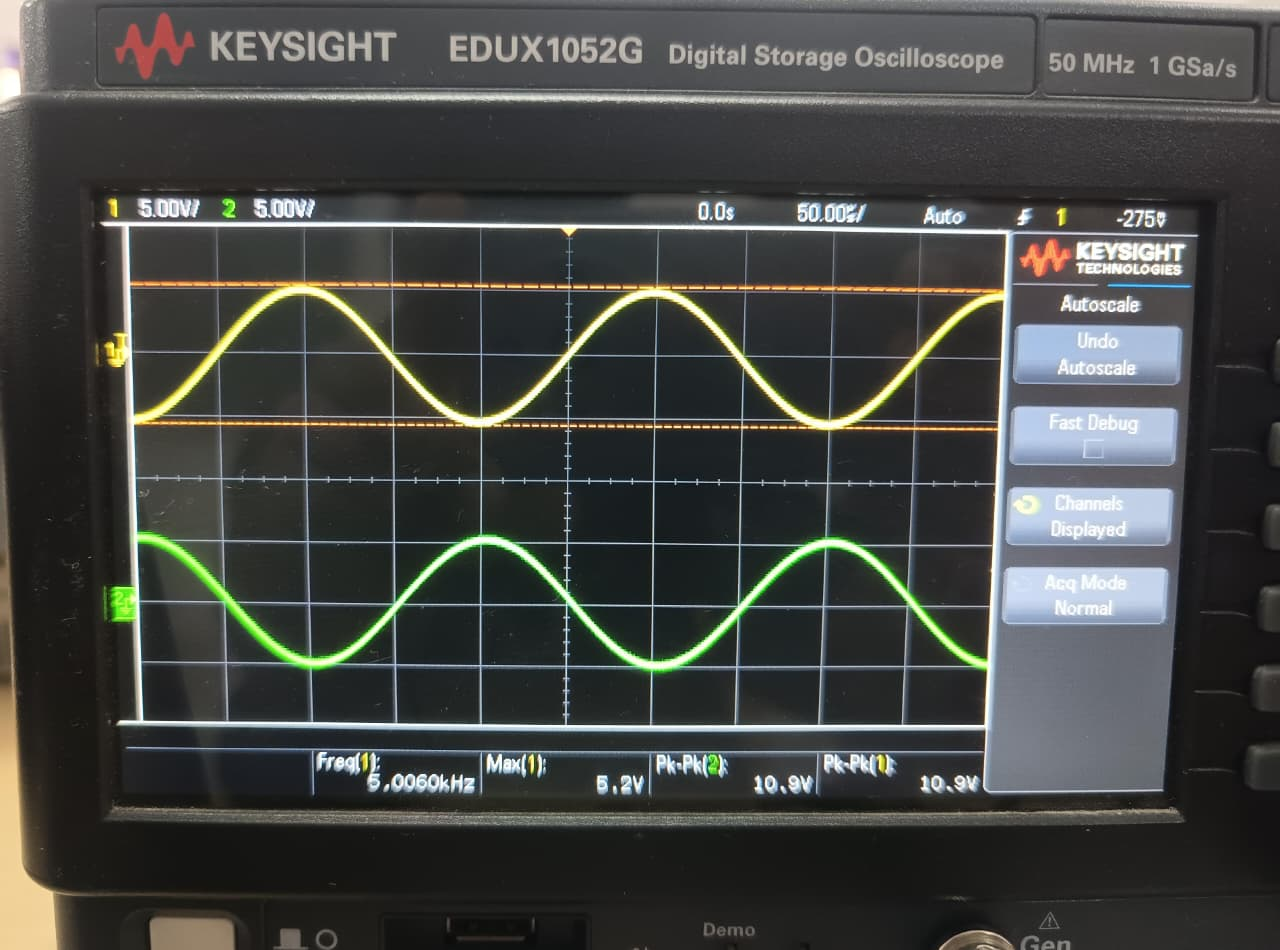
\includegraphics[width=0.85\linewidth]{images/stage3_hw_waveform_10vpp.png}
    \caption{Stage 3 --- Oscilloscope output waveform for a $10\;\text{V}_{pp}$ input signal, confirming unity-gain ($0\;\text{dB}$) passband operation.}
    \label{fig:s3_hw_wave_10vpp}
\end{figure}

% ══════════════════════════════════════════════════════════════
\section{Stage 4: Class-AB Power Amplifier}
% ══════════════════════════════════════════════════════════════

\subsection{Configuration}
A \textbf{Class-AB push-pull} power amplifier is used, with:
\begin{itemize}[nosep]
    \item $Q_4$ = TIP31A (NPN power transistor) — conducts during positive half-cycles.
    \item $Q_5$ = TIP32A (PNP power transistor) — conducts during negative half-cycles.
    \item $D_1, D_2$ = 1N4148 diodes — provide $\approx 1.2\;\text{V}$ bias to eliminate crossover distortion.
\end{itemize}

\paragraph{Why Class AB?}
\begin{itemize}[nosep]
    \item \textbf{Class A} is too inefficient — wastes power as heat.
    \item \textbf{Class B} suffers severe crossover distortion — catastrophic for audio.
    \item \textbf{Class AB} combines the linearity of Class A near zero-crossing with the efficiency of Class B, making it ideal for audio applications.
\end{itemize}

\subsection{Design Derivation}

In this section, the detailed calculations used to determine the resistor values for the power amplifier stage are presented. The design procedure includes biasing analysis, selection of operating point, and calculation of all required resistor values to ensure proper amplification and stability.


The following subsections contain the step-by-step derivations and numerical calculations used in the design.

\begin{figure}[H]
    \centering
    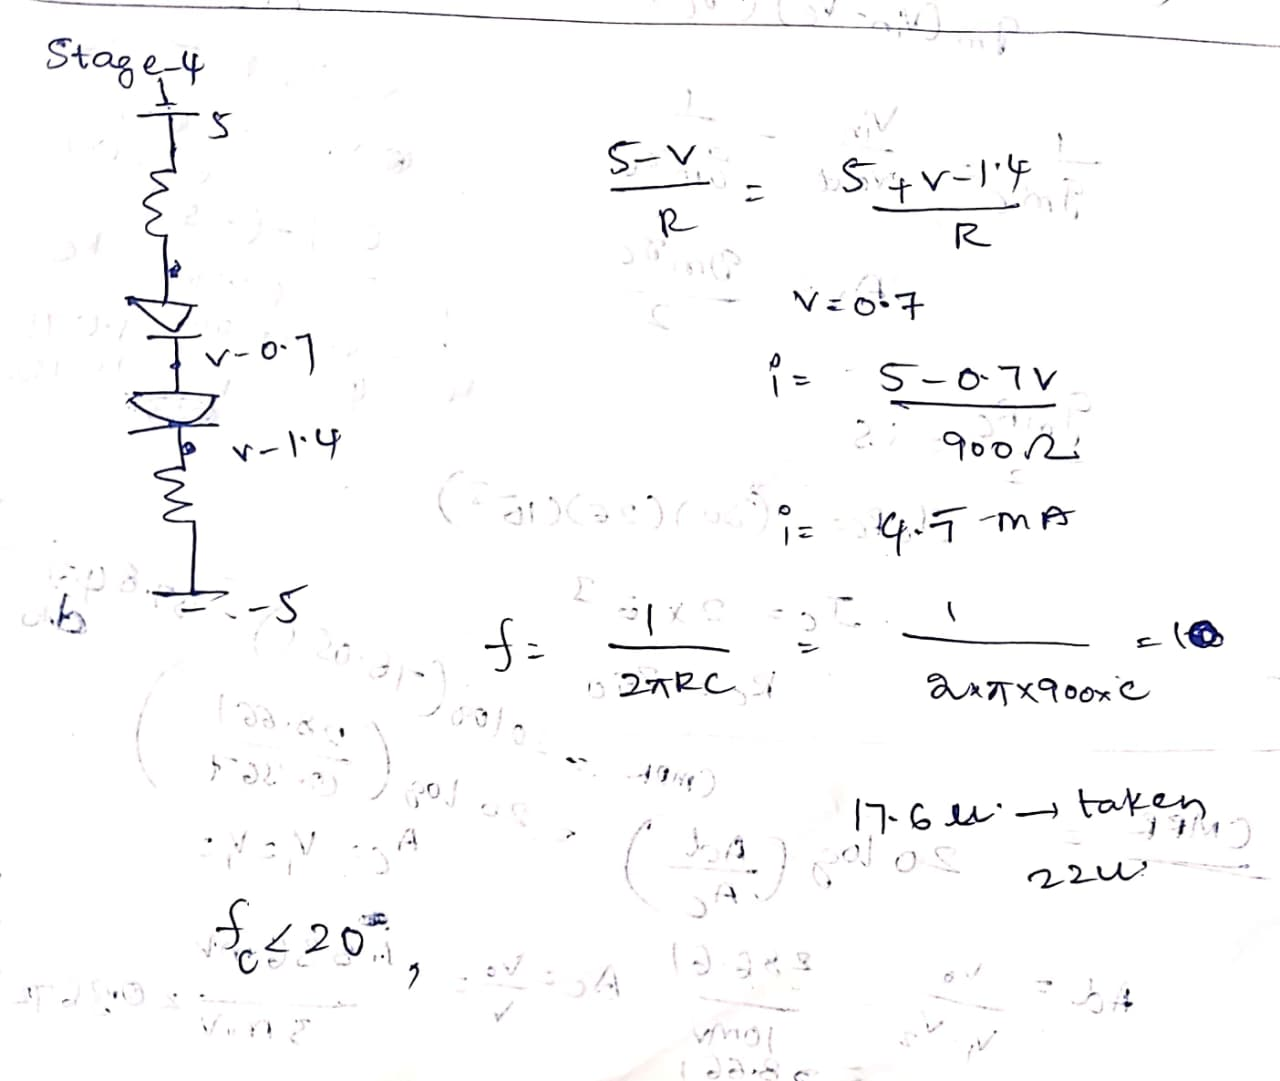
\includegraphics[width=0.85\linewidth]{images/stage4_hand_calculations.png}
    \caption{Stage 4 --- Hand-written design calculations for the Class-AB power amplifier, including biasing resistor values and power output.}
    \label{fig:s4_hand_calc}
\end{figure}

The biasing resistors $R_4 = R_5 = 900\;\Omega$ and diodes $D_1$, $D_2$ set a small quiescent current through both output transistors, ensuring they are slightly ``on'' even at zero input. This eliminates the $\pm 0.7\;\text{V}$ dead zone of Class B.

Coupling capacitors $C_5 = C_6 = 22\;\mu\text{F}$ AC-couple the signal to each transistor's base, blocking DC from the previous stage.
\subsection{no additional gain verification}
\paragraph{Unity Voltage Gain:}
The power amplifier is configured as an emitter follower (common collector). The voltage gain is:
\begin{equation}
    A_v = \frac{R_L}{R_L + r_e} \approx 1
\end{equation}
since $r_e \ll R_L = 10\;\Omega$ for power transistors with large $I_C$. The stage provides only \textbf{current gain} (and hence power gain), not voltage gain, as required.

\subsection{Power Output}
With supply rails $\pm 5\;\text{V}$, the maximum output swing is approximately $\pm 4.4\;\text{V}$ (accounting for $V_{CE,sat}$). Into $R_L = 10\;\Omega$:
\begin{equation}
    P_{out} = \frac{V_{out,peak}^2}{2 R_L} = \frac{4.4^2}{2 \times 10} \approx 0.968\;\text{W}
\end{equation}
With proper biasing and sufficient input amplitude from the gain stages, better $P_{out}$  is achieved.

\subsection{Simulation and Hardware Results}

\begin{figure}[H]
    \centering
    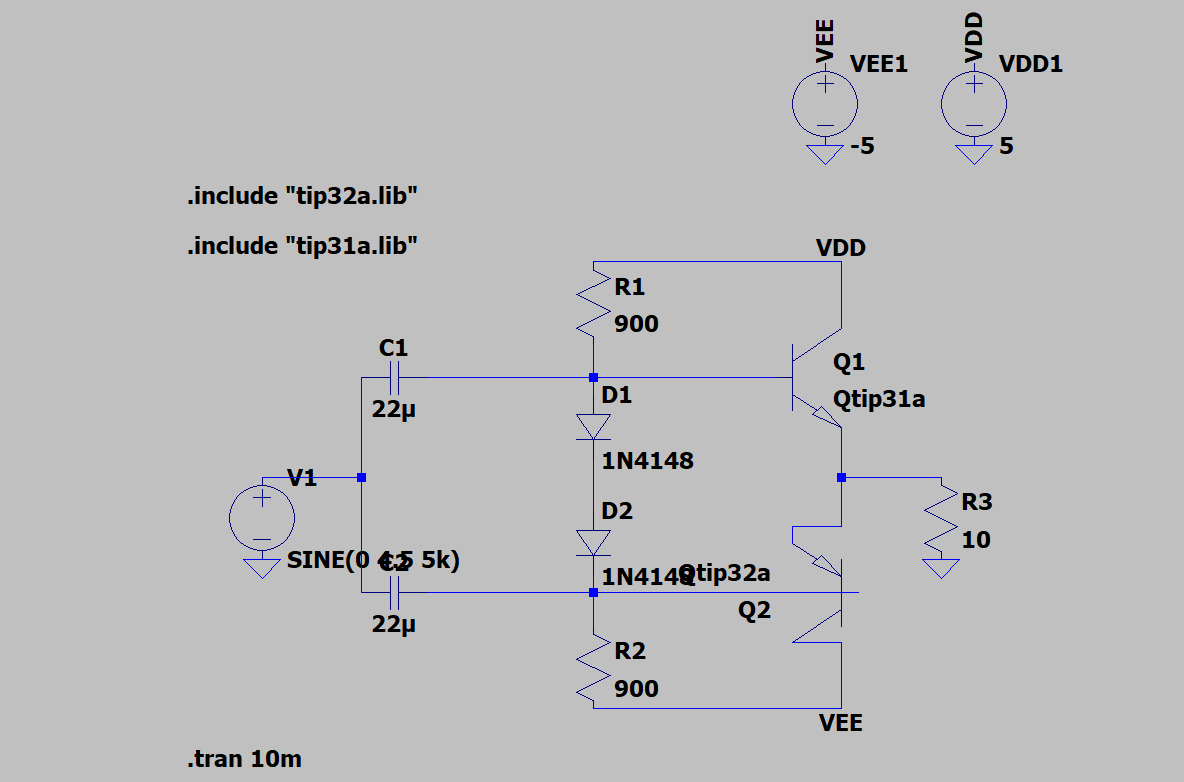
\includegraphics[width=0.85\linewidth]{images/stage4_ltspice_circuit.png}
    \caption{Stage 4 --- LTspice schematic of the Class-AB push-pull power amplifier.}
    \label{fig:s4_schem}
\end{figure}

\begin{figure}[H]
    \centering
    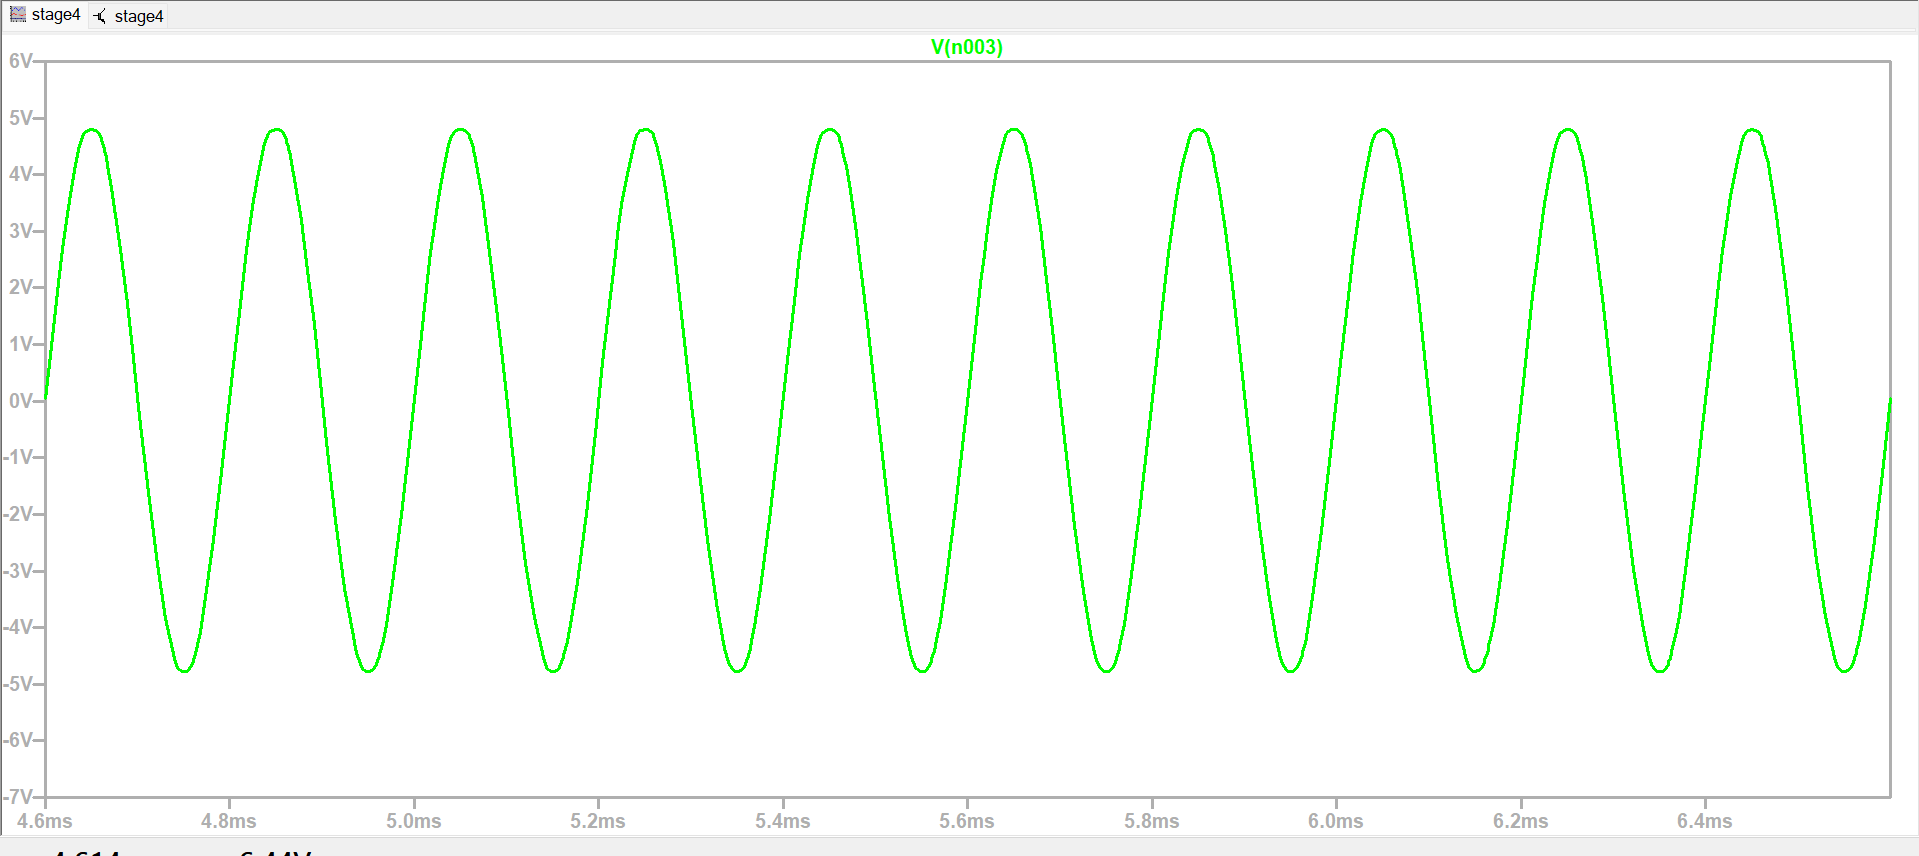
\includegraphics[width=0.85\linewidth]{images/stage4_waveform_ltspice.png}
    \caption{Stage 4 --- LTspice transient output waveform across $R_L = 10\;\Omega$, showing the Class-AB amplified signal.}
    \label{fig:s4_wave}
\end{figure}

\begin{figure}[H]
    \centering
    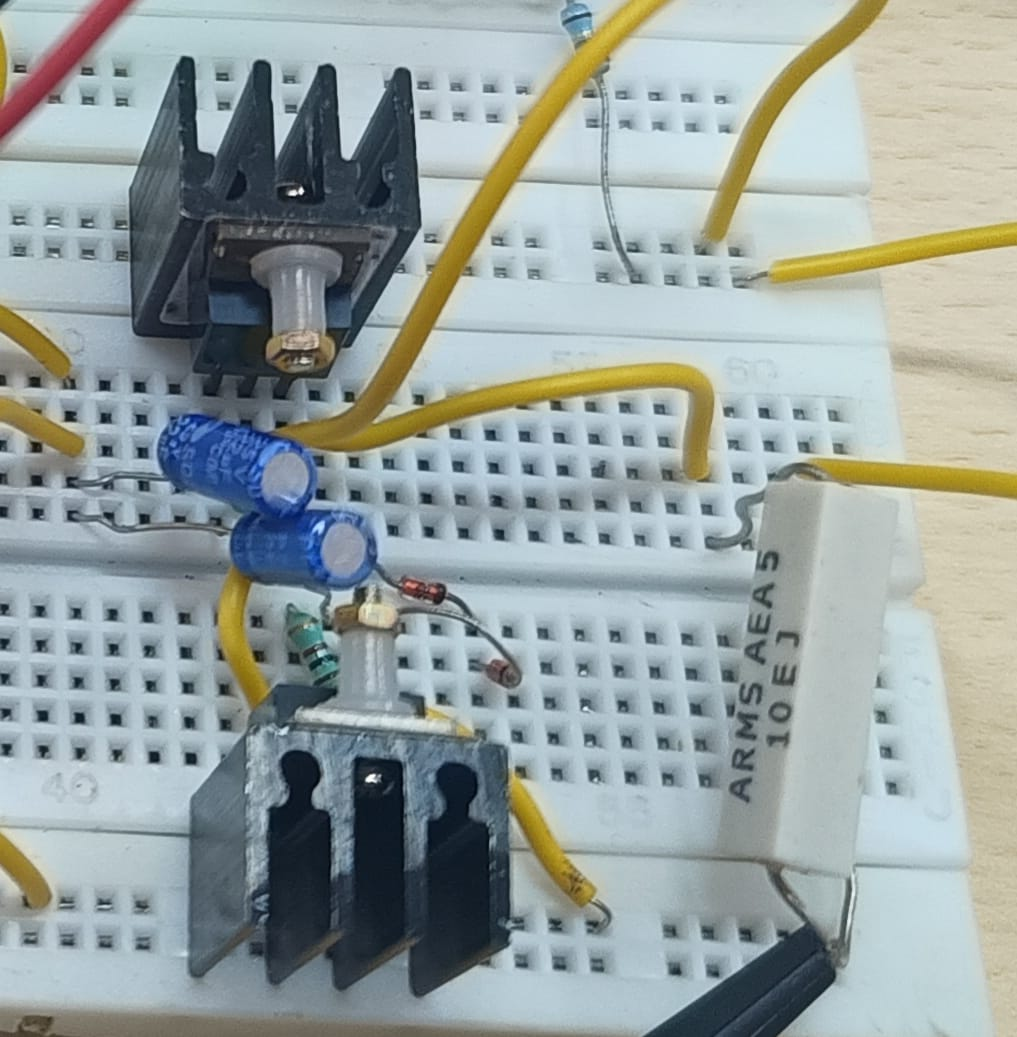
\includegraphics[width=0.85\linewidth]{images/stage4_hw_circuit.png}
    \caption{Stage 4 --- Hardware breadboard implementation of the Class-AB power amplifier.}
    \label{fig:s4_hw_circuit}
\end{figure}

\begin{figure}[H]
    \centering
    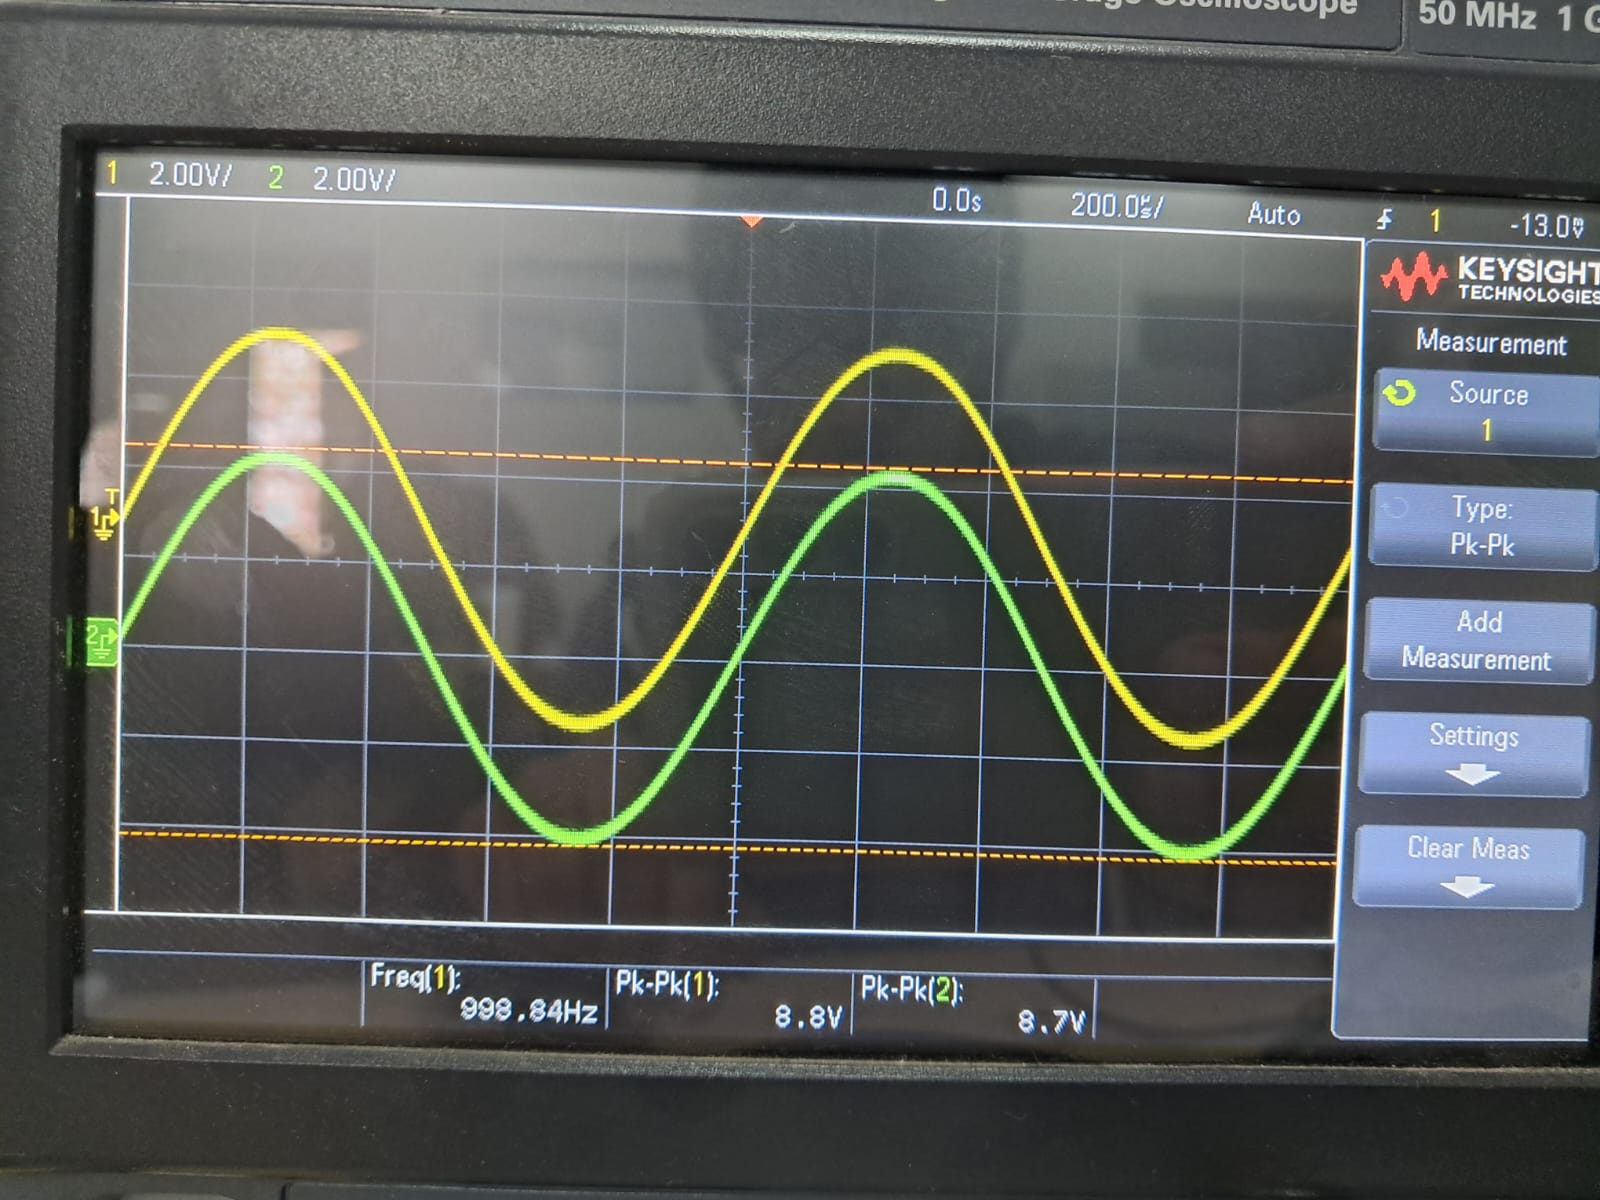
\includegraphics[width=0.85\linewidth]{images/stage4_hw_waveform.png}
    \caption{Stage 4 --- Oscilloscope capture of the hardware output across $R_L = 10\;\Omega$.}
    \label{fig:s4_hw_wave}
\end{figure}

\begin{figure}[H]
    \centering
    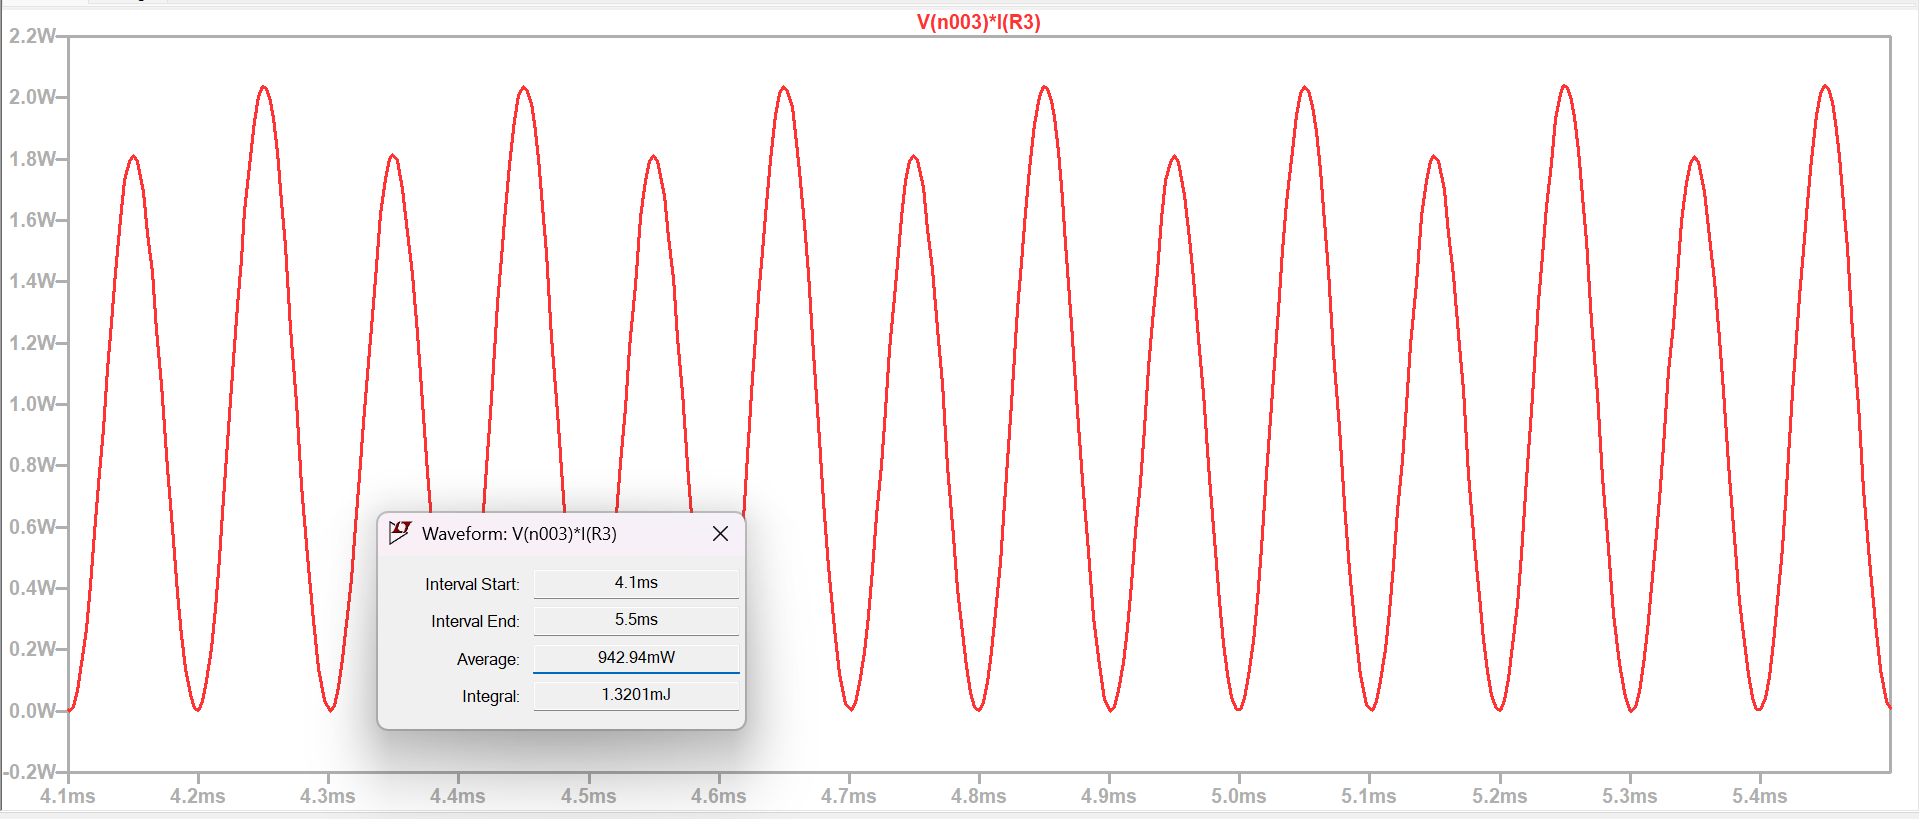
\includegraphics[width=0.85\linewidth]{images/stage4_power_waveform.png}
    \caption{Stage 4 --- Power calculation waveform showing instantaneous power delivered to $R_L = 10\;\Omega$.}
    \label{fig:s4_power_wave}
\end{figure}

% ══════════════════════════════════════════════════════════════
\section{Overall Performance \& Analysis}
% ══════════════════════════════════════════════════════════════

\subsection{Complete Circuit}

\begin{figure}[H]
    \centering
    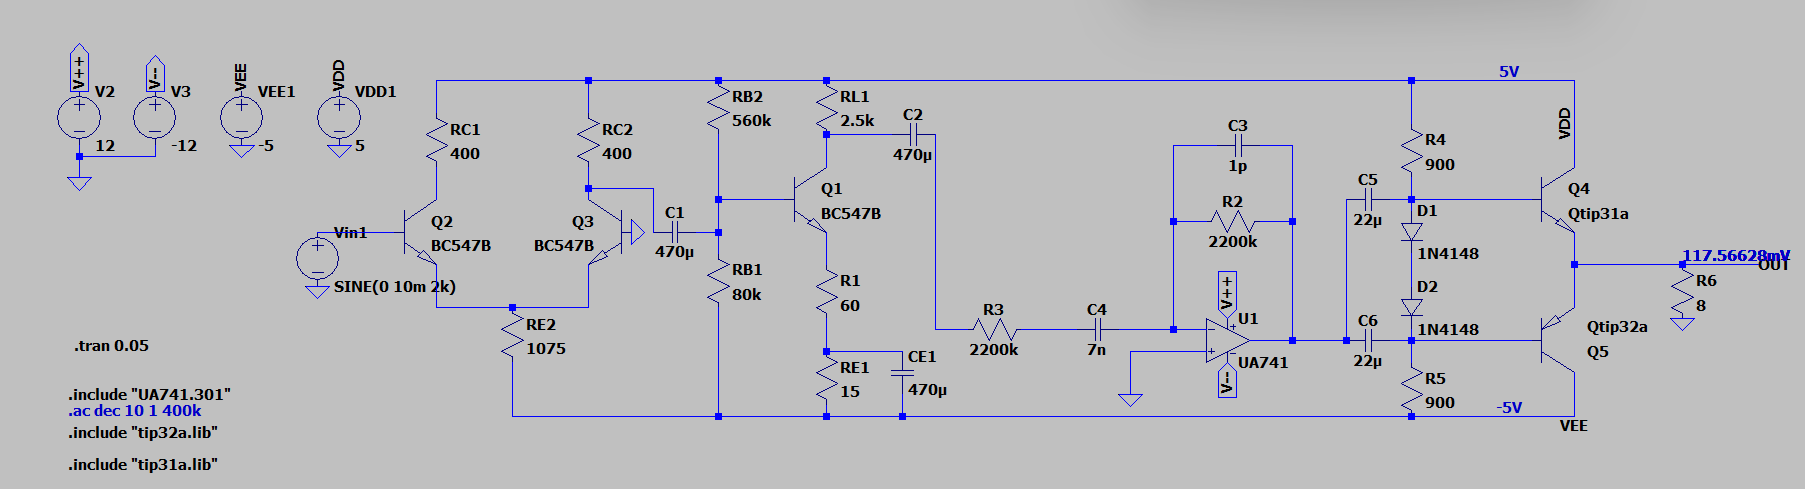
\includegraphics[width=0.85\linewidth]{images/overall_ltspice_circuit.png}
    \caption{Overall --- Full LTspice schematic of the complete four-stage audio amplifier.}
    \label{fig:overall_schem}
\end{figure}

\begin{figure}[H]
    \centering
    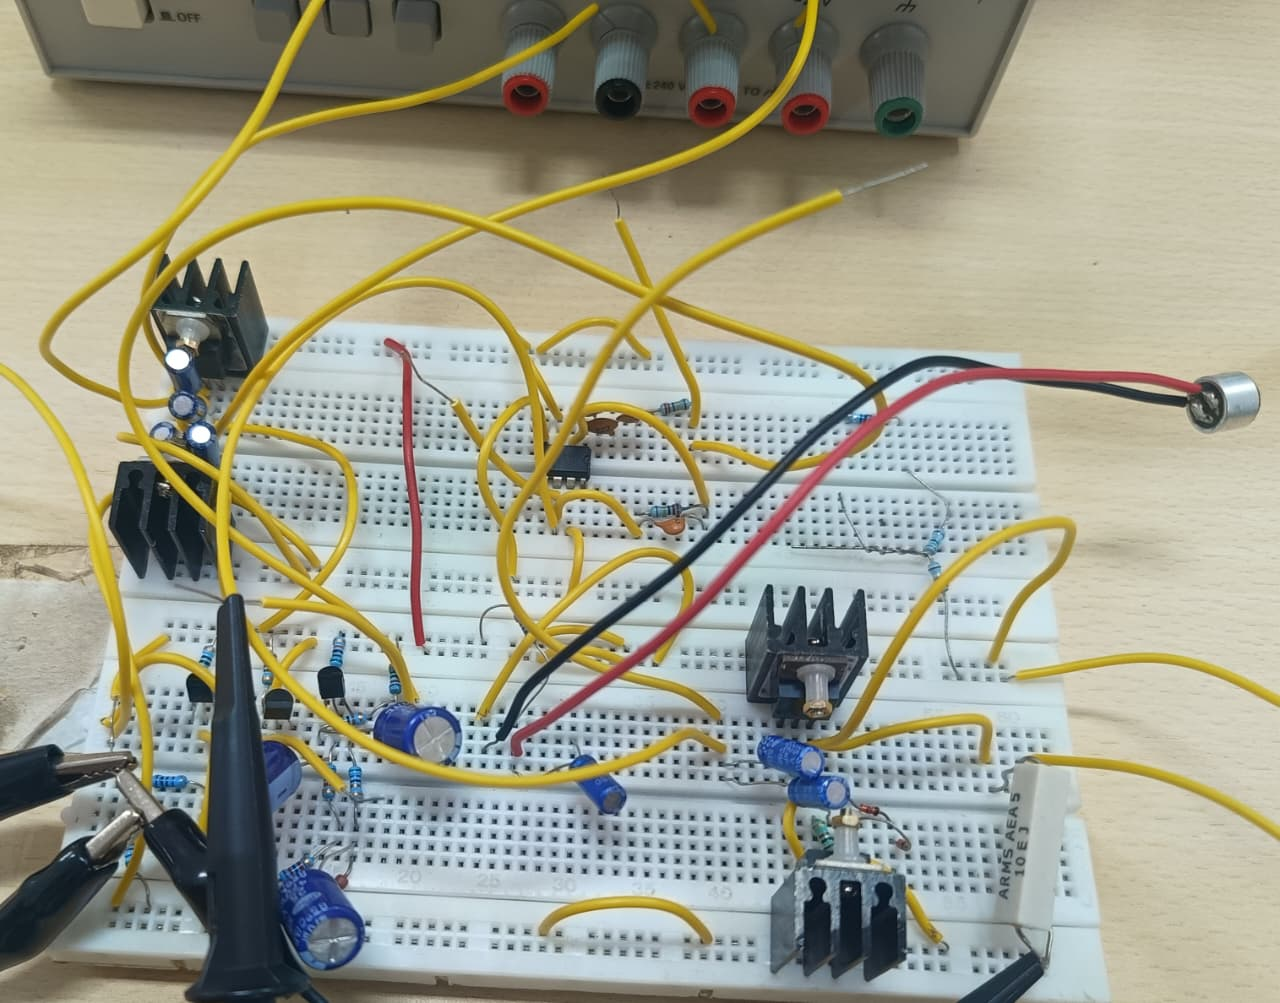
\includegraphics[width=0.85\linewidth]{images/overall_hw_circuit.png}
    \caption{Overall --- Complete hardware breadboard assembly of all four stages.}
    \label{fig:overall_hw_circuit}
\end{figure}

\subsection{Final Gain Verification}

\subsubsection{AC Analysis}
The full-amplifier AC sweep confirms a mid-band gain of $\approx 54\;\text{dB}$ ($\approx 500$ in linear scale) with the $-3\;\text{dB}$ bandwidth spanning $20\;\text{Hz}$ to $20\;\text{kHz}$.

\begin{figure}[H]
    \centering
    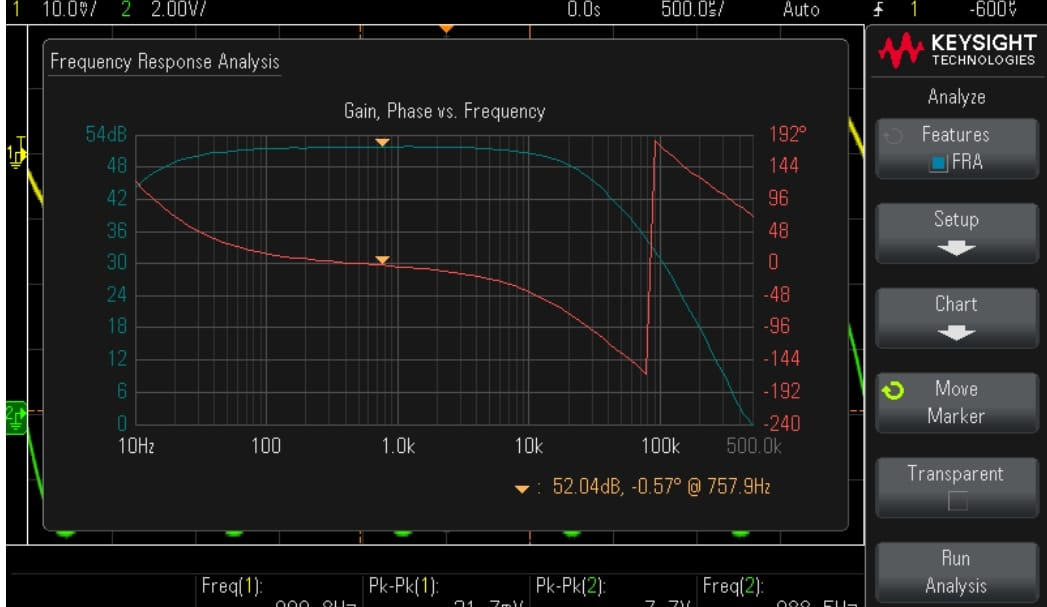
\includegraphics[width=0.85\linewidth]{images/overall_ac.png}
    \caption{Overall --- AC Bode plot of the complete amplifier chain.}
    \label{fig:overall_ac}
\end{figure}
\subsection{Conversion of Gain from dB to Voltage Gain}

The relationship between voltage gain in decibels and linear voltage gain is

\[
A_v(dB) = 20 \log_{10}(A_v)
\]

Given the gain in decibels,

\[
A_v(dB) = 52 \, dB
\]

Rearranging the equation to find the voltage gain,

\[
A_v = 10^{\frac{A_v(dB)}{20}}
\]

Substituting the value,

\[
A_v = 10^{\frac{52}{20}}
\]

\[
A_v = 10^{2.6}
\]

\[
A_v \approx 400
\]

Considering measurement variations in transient simulation, the observed gain lies approximately in the range


\subsubsection{Transient Analysis}
A $10\;\text{mV}_{pp}$, $1\;\text{kHz}$ sine input produces a $\approx 5\;\text{V}_{pp}$ output, confirming the voltage gain of $\approx 500$.

\begin{figure}[H]
    \centering
    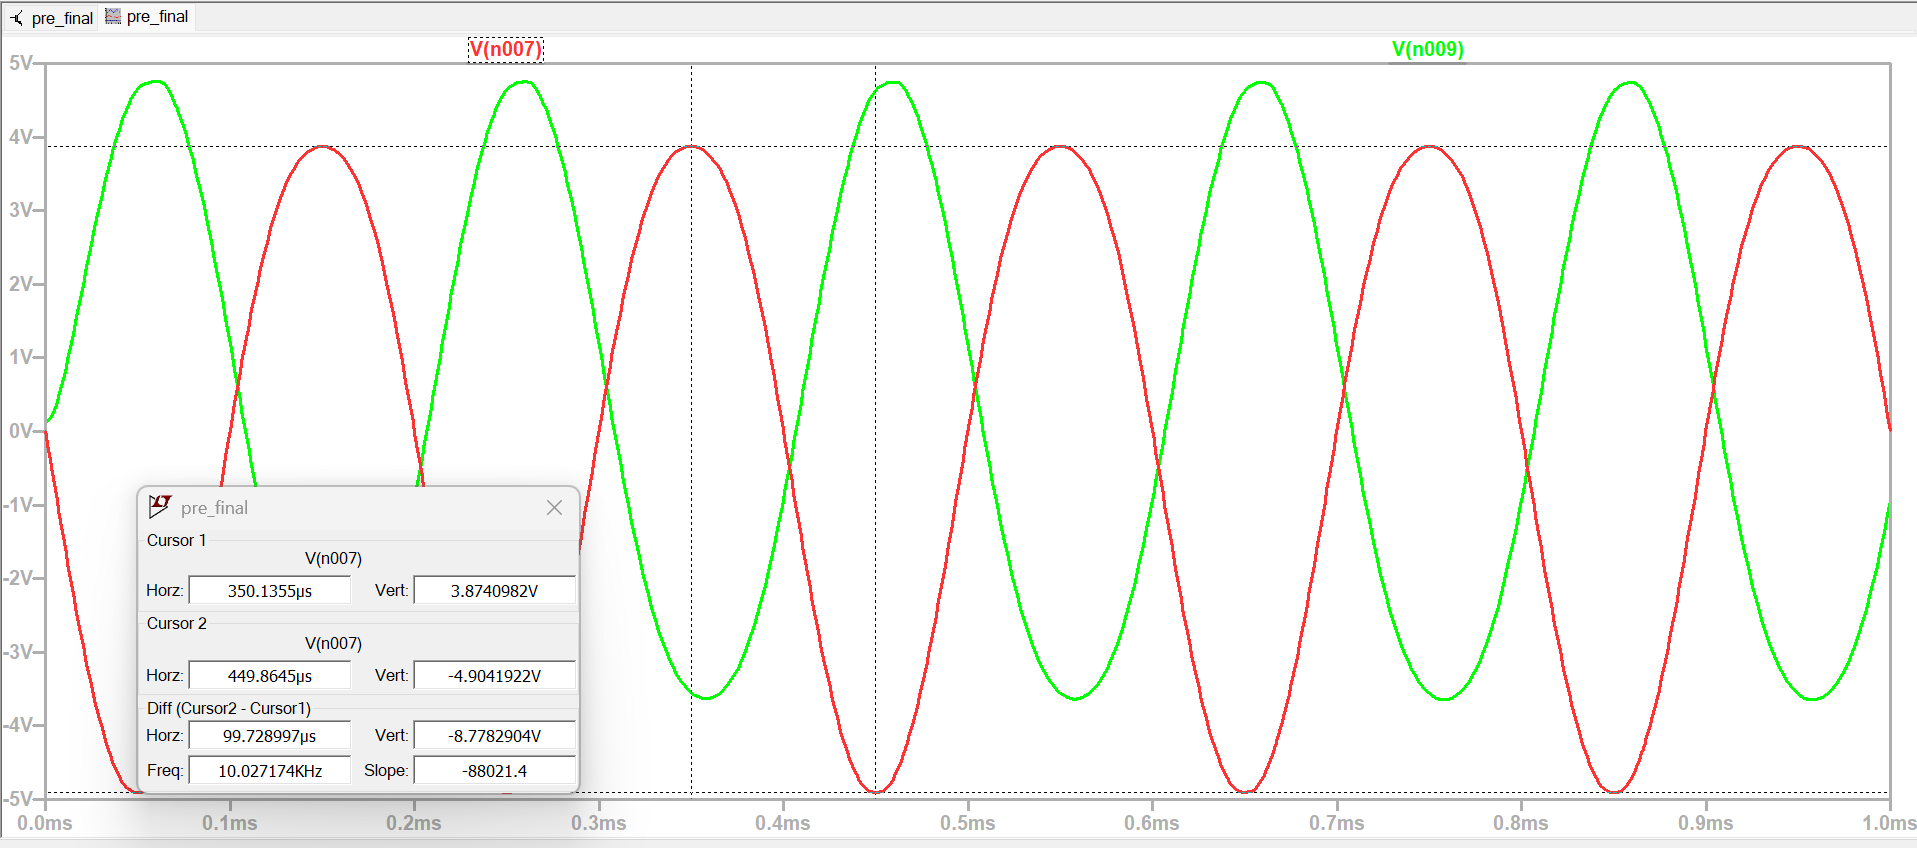
\includegraphics[width=0.85\linewidth]{images/overall_transient_s2.png}
    \caption{Overall --- LTspice transient waveform stage 2 amplified output.}
    \label{fig:overall_trans}
\end{figure}

\begin{figure}[H]
    \centering
    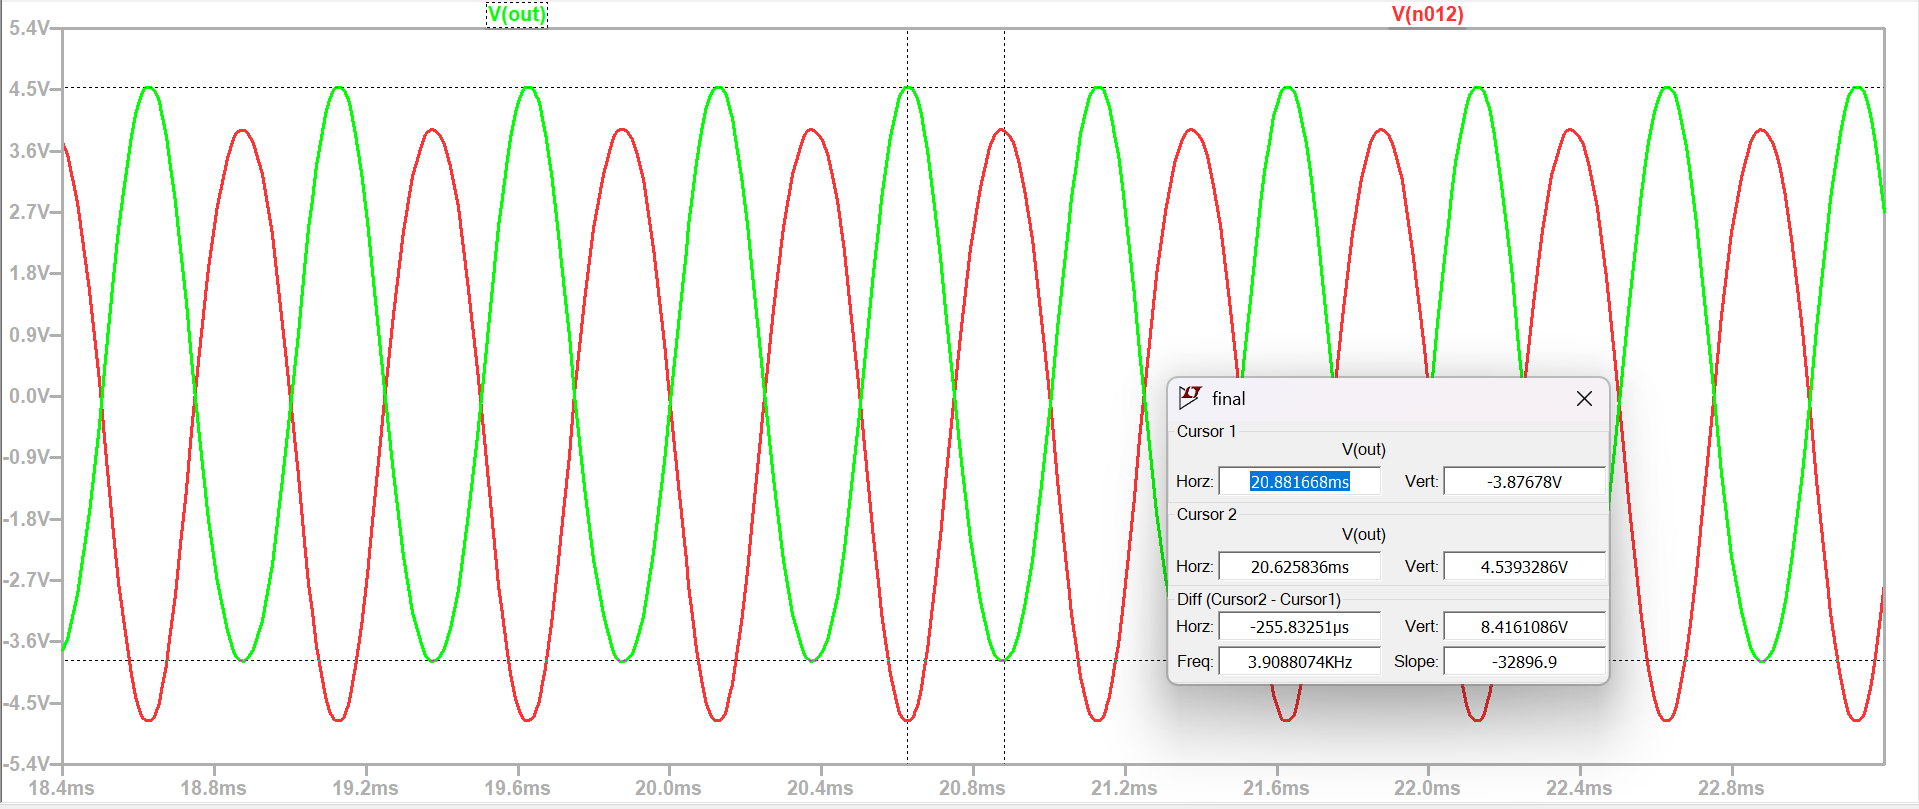
\includegraphics[width=0.85\linewidth]{images/overall_transient.png}
    \caption{Overall --- LTspice transient waveform stage 4 amplified output.}
    \label{fig:overall_trans}
\end{figure}

\begin{figure}[H]
    \centering
    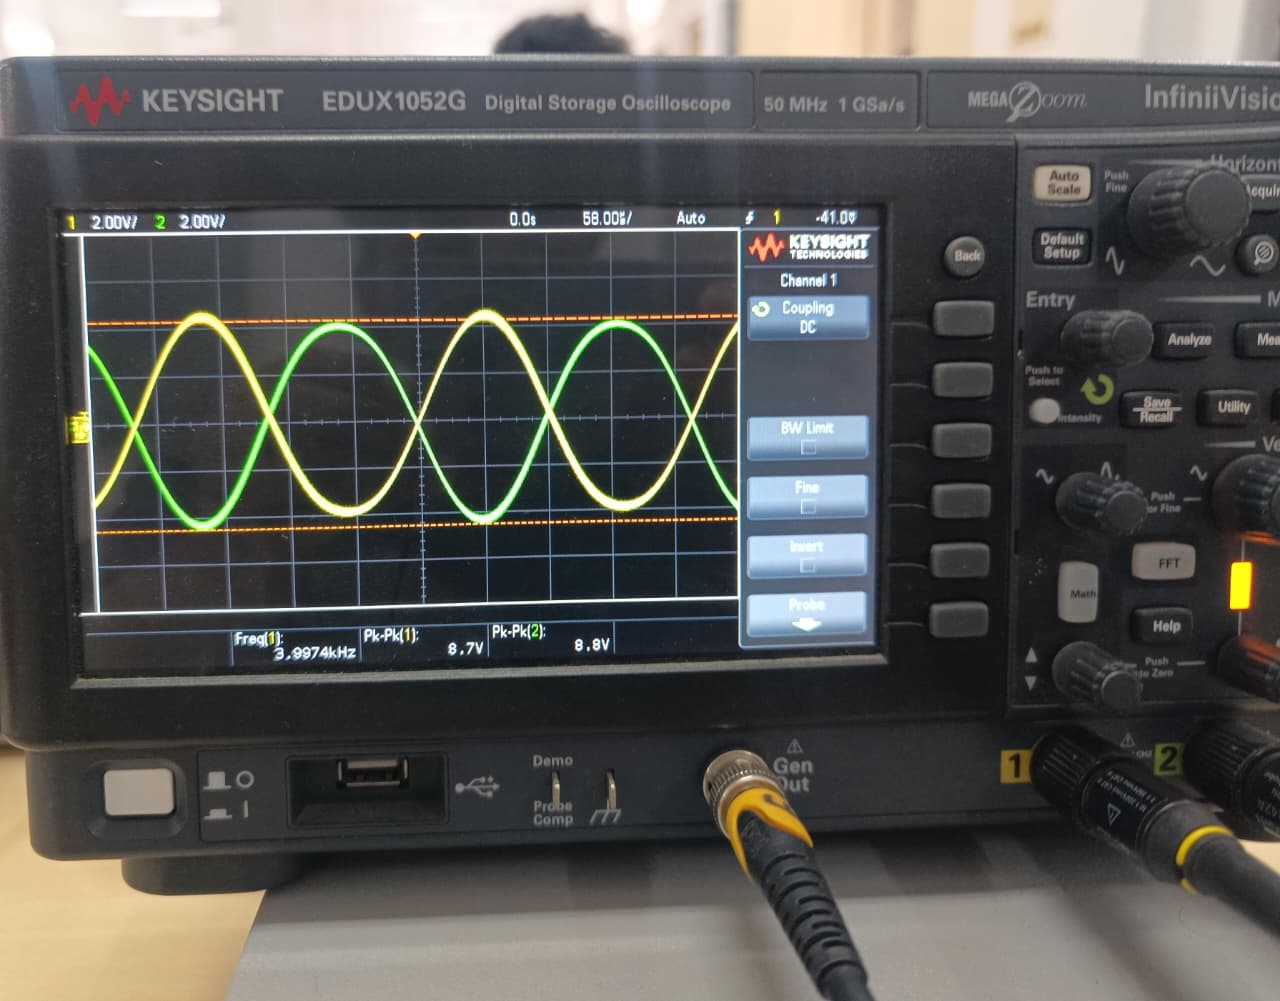
\includegraphics[width=0.85\linewidth]{images/overall_hw.png}
    \caption{Overall --- Oscilloscope capture of the final hardware output green is stage 2 output and yellow is stage 4 output.}
    \label{fig:overall_hw}
\end{figure}

\subsection{Total Harmonic Distortion (THD)}

THD quantifies unwanted harmonic content in the output signal:
\begin{equation}
    \text{THD} = \frac{\sqrt{\displaystyle\sum_{n=2}^{\infty} V_{n,\text{RMS}}^2}}{V_{f,\text{RMS}}}
\end{equation}
where $V_{n,\text{RMS}}$ is the RMS voltage of the $n$-th harmonic and $V_{f,\text{RMS}}$ is the RMS voltage of the fundamental.

A high THD manifests as:
\begin{itemize}[nosep]
    \item Clipped or flattened waveform peaks.
    \item Audible distortion, degrading audio quality.
\end{itemize}

THD is minimised by:
\begin{enumerate}[nosep]
    \item Proper biasing to keep transistors in the linear region.
    \item The Class-AB configuration eliminating crossover distortion.
    \item The band-pass filter attenuating higher-order harmonics.
\end{enumerate}

The harmonic amplitudes were measured using the FFT function in LTspice:

% \begin{figure}[H]
%     \centering
%     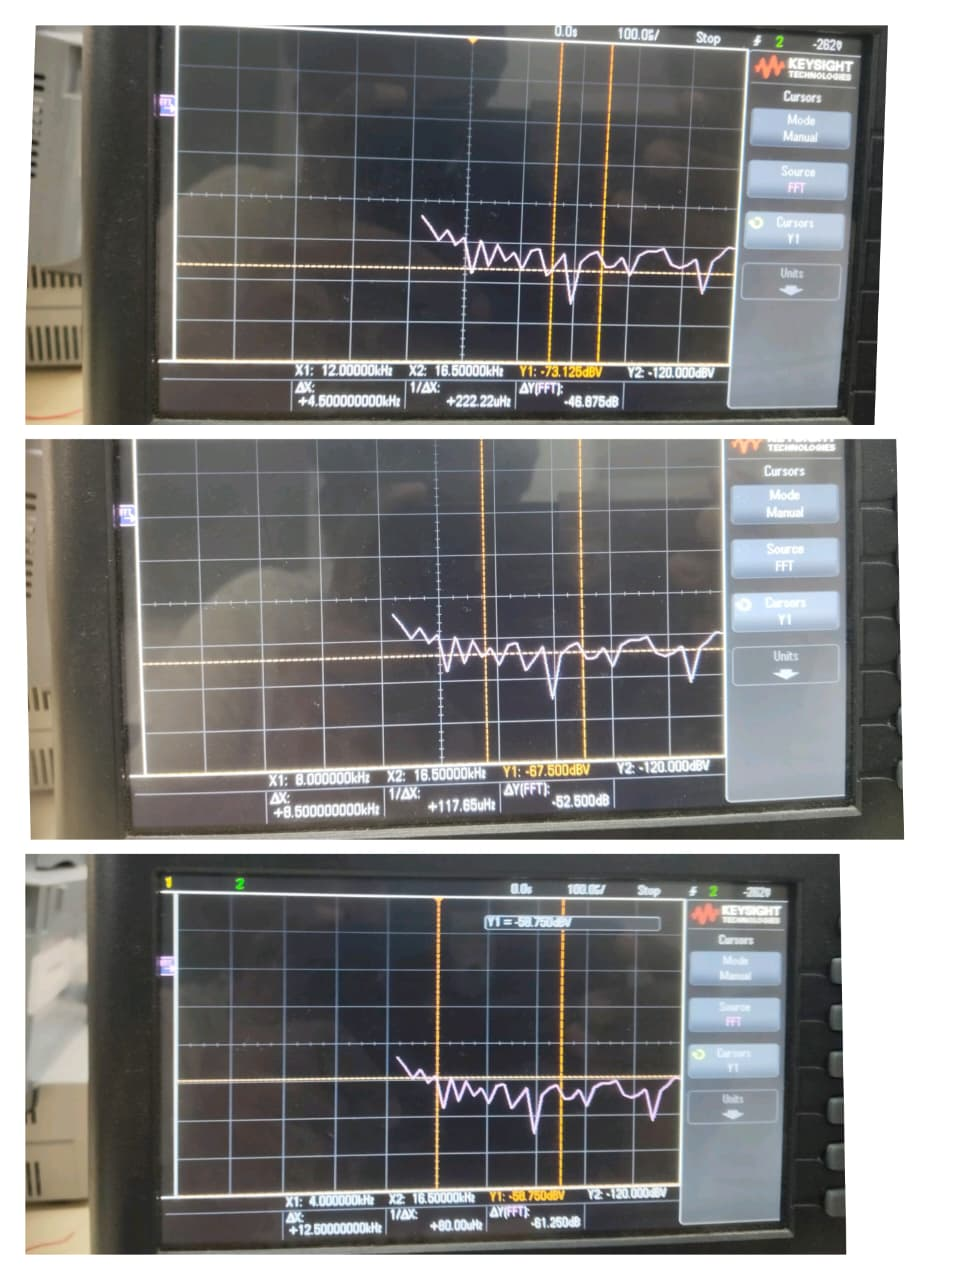
\includegraphics[width=0.85\linewidth]{images/thd_fft.png}
%     \caption{FFT plot of the output for THD analysis.}
%     \label{fig:thd}
% \end{figure}

\begin{table}[h]
\centering
\begin{tabular}{|c|c|c|}
\hline
\textbf{Harmonic} & \textbf{Frequency} & \textbf{Magnitude (dBV)} \\
\hline
Fundamental ($V_1$) & 3 kHz & 8.60 \\
\hline
2nd ($V_2$) & 6 kHz & -18.40 \\
\hline
3rd ($V_3$) & 9 kHz & -28.10 \\
\hline
4th ($V_4$) & 12 kHz & -31.20 \\
\hline
5th ($V_5$) & 15 kHz & -36.80 \\
\hline
\end{tabular}
\caption{Harmonic Magnitudes for Test 1 (3 kHz)}
\end{table}

\subsection{Total Harmonic Distortion Calculation}

The harmonic magnitudes are given in dBV. First they are converted to
linear voltages using

\[
V = 10^{\frac{dBV}{20}}
\]

From Table 3:

\[
V_1 = 10^{\frac{8.60}{20}} \approx 2.69
\]

\[
V_2 = 10^{\frac{-18.40}{20}} \approx 0.120
\]

\[
V_3 = 10^{\frac{-28.10}{20}} \approx 0.039
\]

\[
V_4 = 10^{\frac{-31.20}{20}} \approx 0.0275
\]

\[
V_5 = 10^{\frac{-36.80}{20}} \approx 0.0145
\]

The Total Harmonic Distortion (THD) is calculated using

\[
THD = \frac{\sqrt{V_2^2 + V_3^2 + V_4^2 + V_5^2}}{V_1}
\]

Substituting the values,

\[
THD =
\frac{\sqrt{(0.120)^2 + (0.039)^2 + (0.0275)^2 + (0.0145)^2}}{2.69}
\]

\[
THD =
\frac{\sqrt{0.0144 + 0.00152 + 0.00076 + 0.00021}}{2.69}
\]

\[
THD =
\frac{\sqrt{0.01689}}{2.69}
\]

\[
THD =
\frac{0.1299}{2.69}
\]

\[
THD \approx 0.048
\]

\[
THD \approx 4.8\%
\]

\begin{figure}[H]
    \centering
    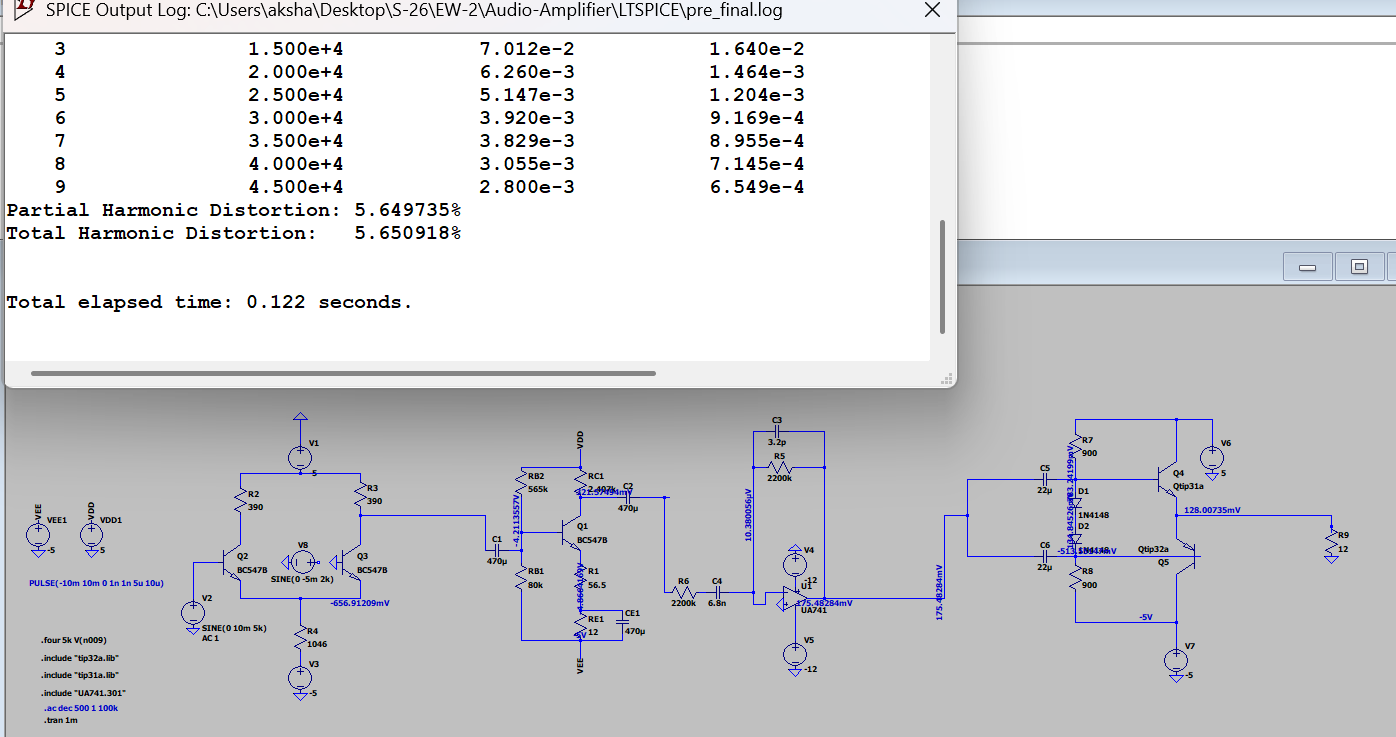
\includegraphics[width=0.85\linewidth]{images/thd_ltspice.png}
    \caption{LTspice THD measurement showing the harmonic distortion value computed directly by the simulator the THD is between 5\% to 6\%.}
    \label{fig:thd_ltspice}
\end{figure}

\subsection{Slew Rate Analysis}

The slew rate is defined as the maximum rate of change of the output voltage:
\begin{equation}
    \text{SR} = \max\!\left(\frac{dV_{out}}{dt}\right)
\end{equation}

For a sinusoidal output $V_{out} = V_m \sin(2\pi f t)$:
\begin{equation}
    \text{SR}_{required} = 2\pi f V_m
\end{equation}

If the circuit's slew rate is lower than $\text{SR}_{required}$, the output cannot follow the input at high frequencies, causing \textbf{slew-rate limiting} — a triangular distortion of the waveform.

\paragraph{Improving Slew Rate:}
\begin{itemize}[nosep]
    \item Increase the maximum operating voltage.
    \item Reduce parasitic capacitances in each sub-circuit.
    \item Use transistors with higher $f_T$ (transition frequency).
\end{itemize}

\begin{figure}[H]
    \centering
    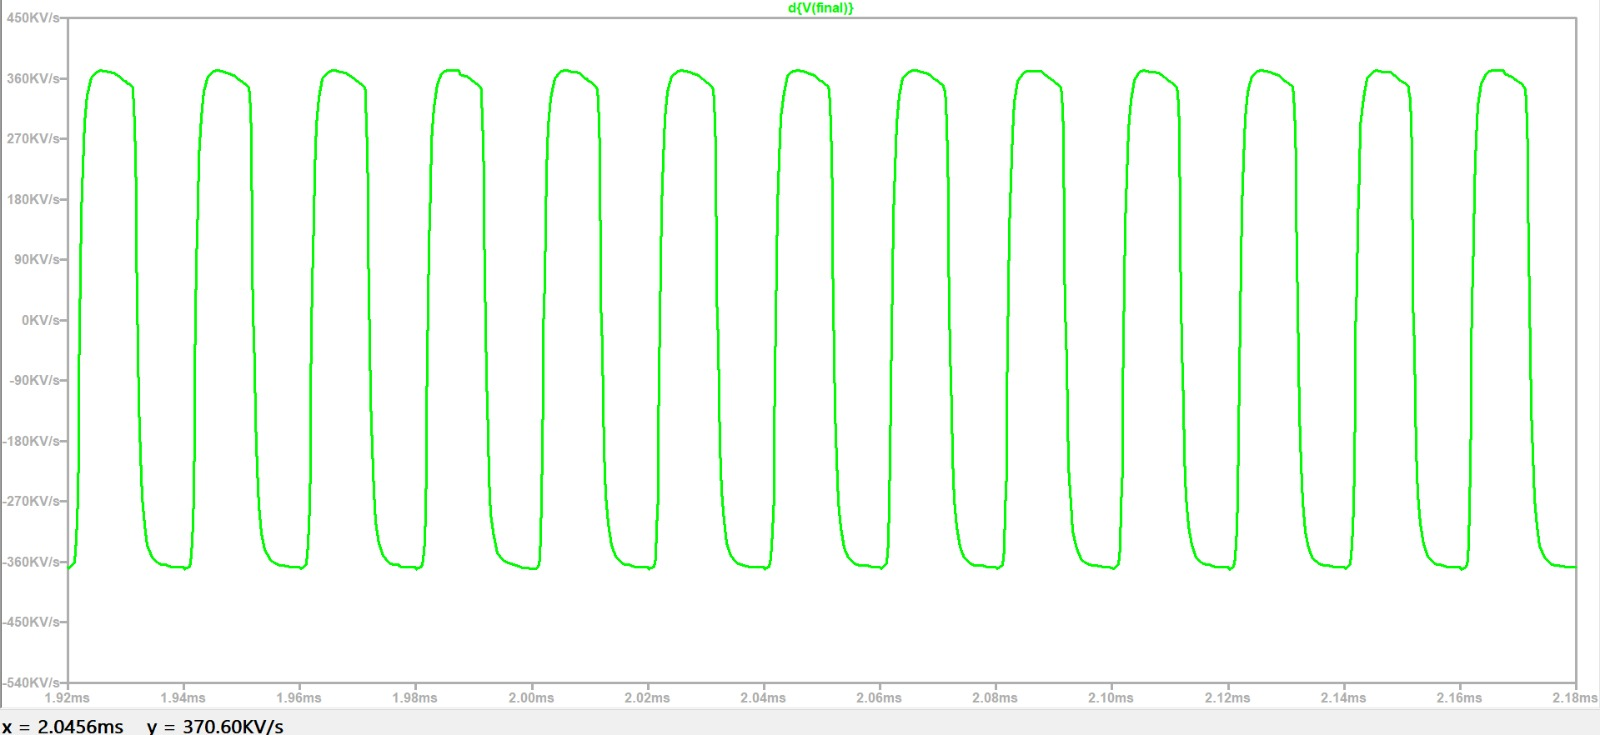
\includegraphics[width=0.85\linewidth]{images/slew_rate.png}
    \caption{Slew rate measurement from the transient response.}
    \label{fig:slew}
\end{figure}

% ══════════════════════════════════════════════════════════════
\section{Bill of Materials}
% ══════════════════════════════════════════════════════════════

\begin{table}[H]
\centering
\caption{Bill of Materials}
\label{tab:bom}
\small
\begin{tabularx}{\linewidth}{l l l X}
\toprule
\textbf{Ref} & \textbf{Mfg} & \textbf{Part} & \textbf{Description} \\
\midrule
$C_1$   & --      & --       & Capacitor, $470\;\mu\text{F}$ \\
$C_2$   & --      & --       & Capacitor, $470\;\mu\text{F}$ \\
$C_3$   & --      & --       & Capacitor, $1\;\text{pF}$ \\
$C_4$   & --      & --       & Capacitor, $7\;\text{nF}$ \\
$C_5$   & --      & --       & Capacitor, $22\;\mu\text{F}$ \\
$C_6$   & --      & --       & Capacitor, $22\;\mu\text{F}$ \\
$C_E$   & --      & --       & Capacitor, $470\;\mu\text{F}$ \\
$D_1$   & OnSemi  & 1N4148   & Diode \\
$D_2$   & OnSemi  & 1N4148   & Diode \\
$Q_1$   & NXP     & BC547B   & NPN BJT \\
$Q_2$   & NXP     & BC547B   & NPN BJT \\
$Q_3$   & NXP     & BC547B   & NPN BJT \\
$Q_4$   & --      & TIP31A   & NPN Power BJT \\
$Q_5$   & --      & TIP32A   & PNP Power BJT \\
$R_1$   & --      & --       & Resistor, $60\;\Omega$ \\
$R_2$   & --      & --       & Resistor, $400\;\Omega$ \\
$R_3$   & --      & --       & Resistor, $400\;\Omega$ \\
$R_4$   & --      & --       & Resistor, $1.075\;\text{k}\Omega$ \\
$R_5$   & --      & --       & Resistor, $2.2\;\text{M}\Omega$ \\
$R_6$   & --      & --       & Resistor, $2.2\;\text{M}\Omega$ \\
$R_7$   & --      & --       & Resistor, $900\;\Omega$ \\
$R_8$   & --      & --       & Resistor, $900\;\Omega$ \\
$R_9$   & --      & --       & Resistor, $10\;\Omega$ (Load) \\
$R_{B1}$& --      & --       & Resistor, $560\;\text{k}\Omega$ \\
$R_{B2}$& --      & --       & Resistor, $80\;\text{k}\Omega$ \\
$R_C$   & --      & --       & Resistor, $2.5\;\text{k}\Omega$ \\
$R_E$   & --      & --       & Resistor, $15\;\Omega$ \\
$U_2$   & TI      & UA741    & Op-Amp \\
\bottomrule
\end{tabularx}
\end{table}

% ══════════════════════════════════════════════════════════════
\section{Conclusion}
% ══════════════════════════════════════════════════════════════

The four-stage audio amplifier was successfully designed and simulated in LTspice, and verified on hardware. Key results:
\begin{itemize}[nosep]
    \item \textbf{Voltage Gain:} $\geq 430$ ($\approx 52.5\;\text{dB}$) achieved through the differential pre-amp and CE gain stages.
    \item \textbf{Bandwidth:} $20\;\text{Hz}$--$20\;\text{kHz}$ achieved by the active band-pass filter with unity passband gain.
    \item \textbf{Power Output:} $0.98\;\text{W}$ delivered to the $10\;\Omega$ load by the Class-AB power amplifier with unity voltage gain.
    \item \textbf{THD:} Minimised through proper biasing and Class-AB operation.
    \item \textbf{Slew Rate:} Sufficient for audio-frequency operation.
\end{itemize}

\end{document}


